% ==============================================================================
% RapidBoxForest (RBF) — IEEE Transactions on Robotics submission source (EN).
% Standalone-compilable from paper/sbf_rbf_only/ while reusing generated assets
% and figures from paper/sbf_old/.
% ==============================================================================
\documentclass[journal]{IEEEtran}

% Load the silence package as early as possible to filter benign font and box
% warnings that are emitted during package/class loading in automated builds.
\RequirePackage{silence}
\WarningFilter{latexfont}{Font shape}
\WarningFilter{latexfont}{Some font shapes were not available}
\hbadness=10000
\vbadness=10000

% Font and micro-typography settings for XeLaTeX: prefer a Times-like
% text font that provides small-caps shapes and reliably defined bold shapes.
% These settings reduce missing-font-shape warnings and improve paragraph
% justification behaviour under XeLaTeX.
\usepackage{fontspec}
% Use the built-in Latin Modern family directly to avoid font discovery work
% during compilation on hosted services.
\setmainfont{Latin Modern Roman}[Ligatures=TeX,Scale=MatchLowercase]
\setsansfont{Latin Modern Sans}[Scale=MatchLowercase]
\setmonofont{Latin Modern Mono}[Scale=MatchLowercase]

% If the document uses \textsc extensively but the chosen font lacks OpenType
% small-caps, avoid generating TU/.../sc requests by mapping \textsc to an
% uppercase form instead of real small-caps shapes. Use a robust definition
\DeclareRobustCommand{\textsc}[1]{\textnormal{\MakeUppercase{#1}}}

% Loosen paragraph tolerance slightly to avoid underfull hbox warnings in
% narrow IEEE two-column layout while keeping good justification.
\tolerance=2000
\emergencystretch=2em
% Keep floats close to the text that introduces them.
\setcounter{topnumber}{4}
\setcounter{bottomnumber}{3}
\setcounter{totalnumber}{6}
\renewcommand{\topfraction}{0.92}
\renewcommand{\bottomfraction}{0.8}
\renewcommand{\textfraction}{0.05}
\renewcommand{\floatpagefraction}{0.85}
\renewcommand{\dbltopfraction}{0.9}
\renewcommand{\dblfloatpagefraction}{0.85}
\setlength{\textfloatsep}{5pt plus 1pt minus 2pt}
\setlength{\dbltextfloatsep}{6pt plus 1pt minus 2pt}
\setlength{\floatsep}{4pt plus 1pt minus 2pt}
\setlength{\intextsep}{5pt plus 1pt minus 2pt}
\setlength{\abovecaptionskip}{3pt}
\setlength{\belowcaptionskip}{0pt}
\setlength{\abovedisplayskip}{5pt plus 1pt minus 2pt}
\setlength{\belowdisplayskip}{5pt plus 1pt minus 2pt}
\setlength{\abovedisplayshortskip}{4pt plus 1pt minus 2pt}
\setlength{\belowdisplayshortskip}{4pt plus 1pt minus 2pt}
\setlength{\jot}{1pt}

\usepackage{amsmath,amssymb,amsfonts}
\usepackage{amsthm}
\usepackage{algorithm}
\usepackage{algorithmic}
\usepackage{afterpage}
\usepackage{booktabs}
\usepackage{dblfloatfix}
\usepackage{rotating}
\usepackage{graphicx}
\usepackage{capt-of}
\usepackage{placeins}
\usepackage{bm}
\usepackage{xr}
\usepackage{hyperref}
\usepackage{cleveref}
\usepackage{etoolbox}
\usepackage[inline]{enumitem}

\newtheorem{theorem}{Theorem}
\newtheorem{proposition}{Proposition}
\newtheorem{definition}{Definition}
\newtheorem{remark}{Remark}
\newtheorem{lemma}{Lemma}
\newtheorem{corollary}{Corollary}
\newtheorem{assumption}{Assumption}

\input{../sbf_old/generated/macros.tex}
\IfFileExists{../sbf_old/generated/macros_sbf.tex}{\input{../sbf_old/generated/macros_sbf.tex}}{}
\IfFileExists{../sbf_old/generated/tro_macros.tex}{% Auto-generated by experiments/tro2026_generate_tables.py
\newcommand{\TroAuditedGcsAuditPass}{--/--}
\newcommand{\TroExpandedGcsAuditPass}{--/--}
\newcommand{\TroDirectGcsAuditPass}{--/--}
\newcommand{\TroSbfBuildMean}{--}
\newcommand{\TroSbfBoxMean}{--}
\newcommand{\TroPaperAuditPass}{--/--}
\newcommand{\TroRbfOnlyEFiveLeafFk}{--}
\newcommand{\TroRbfOnlyEFiveEvidence}{--}
\newcommand{\TroRbfOnlyEFiveFirstWall}{--}
\newcommand{\TroRbfOnlyEFiveReopenWall}{--}
\newcommand{\TroRbfOnlyEFiveReopenReuse}{--}
\newcommand{\TroRbfOnlySweepBestEnvelope}{--}
\newcommand{\TroRbfOnlySweepBestBudget}{--}
\newcommand{\TroRbfOnlySweepBestBuild}{--}
\newcommand{\TroRbfOnlySweepBestQueryMs}{--}
\newcommand{\TroRbfOnlySweepBestReuse}{--}
\newcommand{\TroRbfOnlySweepFullPassRows}{--}
\newcommand{\TroRbfOnlyShelfWarmBuild}{--}
\newcommand{\TroRbfOnlyShelfWarmQueryMs}{--}
\newcommand{\TroRbfOnlyShelfWarmExternalReuse}{--}
\newcommand{\TroRbfOnlyEFourWarmBuildMin}{--}
\newcommand{\TroRbfOnlyEFourWarmBuildMax}{--}
\newcommand{\TroRbfOnlyEFourWarmQueryMinMs}{--}
\newcommand{\TroRbfOnlyEFourWarmQueryMaxMs}{--}
\newcommand{\TroRbfOnlyEFourWarmAuditMin}{--}
\renewcommand{\TroAuditedGcsAuditPass}{3/5}
\renewcommand{\TroExpandedGcsAuditPass}{0/4}
\renewcommand{\TroDirectGcsAuditPass}{0/5}
\renewcommand{\TroSbfBuildMean}{0.9393}
\renewcommand{\TroSbfBoxMean}{150.90}
\renewcommand{\TroPaperAuditPass}{663/668}
\renewcommand{\TroRbfOnlyEFiveLeafFk}{262144}
\renewcommand{\TroRbfOnlyEFiveEvidence}{524287}
\renewcommand{\TroRbfOnlyEFiveFirstWall}{20.17}
\renewcommand{\TroRbfOnlyEFiveReopenWall}{1.505}
\renewcommand{\TroRbfOnlyEFiveReopenReuse}{262144}
\renewcommand{\TroRbfOnlySweepBestEnvelope}{LinkIAABB}
\renewcommand{\TroRbfOnlySweepBestBudget}{256}
\renewcommand{\TroRbfOnlySweepBestBuild}{0.0032}
\renewcommand{\TroRbfOnlySweepBestQueryMs}{46.05}
\renewcommand{\TroRbfOnlySweepBestReuse}{205.00}
\renewcommand{\TroRbfOnlySweepFullPassRows}{6}
\renewcommand{\TroRbfOnlyShelfWarmBuild}{1.588}
\renewcommand{\TroRbfOnlyShelfWarmQueryMs}{3.568}
\renewcommand{\TroRbfOnlyShelfWarmExternalReuse}{7201}
\renewcommand{\TroRbfOnlyEFourWarmBuildMin}{0.0016}
\renewcommand{\TroRbfOnlyEFourWarmBuildMax}{0.5569}
\renewcommand{\TroRbfOnlyEFourWarmQueryMinMs}{0.6615}
\renewcommand{\TroRbfOnlyEFourWarmQueryMaxMs}{3.536}
\renewcommand{\TroRbfOnlyEFourWarmAuditMin}{100.00}
}{}

\newcommand{\rbf}{\textsc{RBF}}
\newcommand{\iAABB}{\ensuremath{\mathrm{iAABB}}}
\newcommand{\Real}{\ensuremath{\mathbb{R}}}
\newcommand{\Cfree}{\ensuremath{\mathcal{C}_{\mathrm{free}}}}
\newcommand{\calO}{\ensuremath{\mathcal{O}}}
\newcommand{\Q}{\ensuremath{\mathcal{Q}}}
\newcommand{\etal}{\textit{et al.}}
\renewcommand{\algorithmicrequire}{\textbf{Input:}}
\renewcommand{\algorithmicensure}{\textbf{Output:}}
\newcommand{\algcommentline}[1]{\STATE \textit{#1}}
\newcommand{\procname}[1]{\operatorname{#1}}

\newcommand{\TableFontStepUp}{%
  \let\TableOrigTiny\tiny
  \let\TableOrigScriptSize\scriptsize
  \let\TableOrigFootnoteSize\footnotesize
  \let\TableOrigSmall\small
  \renewcommand{\tiny}{\TableOrigScriptSize}
  \renewcommand{\scriptsize}{\TableOrigFootnoteSize}
  \renewcommand{\footnotesize}{\TableOrigSmall}
  \renewcommand{\small}{\normalsize}
}
\AtBeginEnvironment{table}{\TableFontStepUp}
\AtBeginEnvironment{table*}{\TableFontStepUp}
\AtBeginEnvironment{sidewaystable}{\TableFontStepUp}

\begin{document}

\title{RapidBoxForest:\\ Link-Envelope-Guided Box Forests for Fast Multi-Query Manipulation}

\author{TIAN,~Yu and Ren,~Hongliang%
\thanks{The authors are with the Department of Electronic Engineering,
The Chinese University of Hong Kong (CUHK), Hong Kong SAR, China.
E-mail: \texttt{ty1997@link.cuhk.edu.hk}.}}

\maketitle

\begin{abstract}
Fast repeated-query manipulation benefits from reusable volumetric planning
structure, but high-quality IRIS-style convex regions are expensive to construct
and rebuild. This paper presents RapidBoxForest (\rbf{}), a link-envelope-guided
box-forest planner for fast multi-query manipulation. The central geometric primitive maps endpoint interval envelopes to link
interval envelopes via capsule Minkowski decomposition and convex-hull generator
bounding applied to \emph{$C$-space box validation and multi-query reuse}:
endpoint interval envelopes bound rounded-link endpoint motion over a joint box,
and a radius-lifted link envelope provides an inexpensive filter for box
validation and collision rejection. A rapidly-exploring random tree
(RRT)-inspired grower builds a scene-specific box forest into a queryable
corridor graph, and a Lifelong Envelope Cache Tree (LECT) selectively caches
kinematics-keyed envelope records when replay is cheaper than recomputation. In
the regenerated endpoint-envelope experiment, each source is evaluated on 6000
shared IIWA14 joint boxes, with 1000 boxes at each of six fixed widths. The
public IFK spelling, which now subsumes the former AAFK alias, averages
4.53~$\mu$s per endpoint box with no observed reference under-coverage.
Hierarchical IFK tightens the mean endpoint volume by up to 76.0\% relative to
IFK at 72.2~$\mu$s. CritSample and MC give smaller boxes but are
non-certified and show observed under-coverage against the finite reference
union. These results bound the quantitative claims in this version to the
endpoint-envelope primitive; full planner-level cache, dynamic-update, and
cross-planner tables are not carried forward here.
\end{abstract}

\begin{IEEEkeywords}
Motion planning, multi-query planning, link interval envelopes, box-region planning, final audit.
\end{IEEEkeywords}

% ==============================================================================
\section{Introduction}\label{sec:intro}

Motion planning for high-degree-of-freedom (DOF) manipulators becomes
especially demanding when a system must answer many related queries rather than
one isolated instance. In warehouses, packing cells, and shared workcells,
robot kinematics stay fixed while obstacles, task endpoints, or local scene
edits change. The central question is how to construct reusable $C$-space
planning structure quickly enough that repeated queries can benefit from
region-level search without paying a large scene-specific preprocessing cost.

Iterative Regional Inflation by Semidefinite Programming (IRIS) and
Graph-of-Convex-Sets (GCS) methods show why free-region construction is
valuable: once good convex regions are available, graph search or convex
optimization can produce high-quality motions over those regions
\cite{deits2015computing,marcucci2023motion,marcucci2024shortest}. The
limitation is construction cost. In high-dimensional manipulator scenes,
inflating and validating high-quality convex regions can dominate the planning
budget and must often be repeated when the scene changes. Sampling-based planners such as probabilistic roadmap (PRM) and
rapidly-exploring random tree (RRT) methods avoid this region-construction cost
\cite{lavalle2006planning,lavalle1998rapidly,kavraki1996probabilistic,
karaman2011sampling}, but their reusable structures are usually zero-volume
graphs, so repeated queries still pay for local collision checking and do not
obtain a reusable free-region cover.

\rbf{} targets a different design point by constructing simpler box regions
quickly.
Instead of inflating general polytopes, it grows axis-aligned boxes in
configuration space, connects accepted boxes into a graph, and answers later
queries by searching the resulting box corridor. This trades per-region
expressivity and sometimes path length for cheap construction, simple
adjacency, and direct reuse across many queries. The intended claim is a
system-level one: a fast box-region planning pipeline can be a useful
final-audited alternative when multi-query latency matters more than obtaining
the shortest path from a more expensive region decomposition.

The key technical ingredient is a link interval envelope computed from endpoint
interval envelopes. For rounded link models, \rbf{} reduces link motion over a
joint box to the motion of a zero-radius centerline plus a final radius lift.
Endpoint interval envelopes bound the endpoint trajectories over the joint box;
link interval envelopes then enclose the swept rounded link and can be stored as
axis-aligned bounding boxes (AABBs), $k$-DOP slabs, or SupportHull records. Strict interval sources provide an
optional conservative validation path, while tighter practical sources are used
as fast filters and discharged by the same final scene audit used for all
reported planners.

On top of this geometric primitive, the grower borrows the rapid
frontier-expansion idea of RRT: samples choose useful frontiers, a local region
oracle materializes a free box around the projected seed, and accepted boxes
extend a connected box forest. The result is also an adaptive cell-decomposition
view of manipulator $C$-space, but one biased toward the regions needed by the
current repeated-query workload. A Lifelong Envelope Cache Tree (LECT) then memoizes scene-independent endpoint
and link-envelope evidence keyed by robot kinematics and joint intervals; it is
an acceleration layer for repeated materialization, not a separate planning
claim.

The evaluation therefore asks how the endpoint-envelope source family behaves
under the adopted protocol. The current quantitative axes are endpoint
construction time, endpoint AABB volume, and the observed under-coverage gap
against a finite reference union on shared IIWA14 joint boxes. Planner-level
cache, dynamic-update, cross-planner, and multi-robot generalization studies
remain future work for this paper track.

We therefore position the paper as a planning-systems contribution enabled by a
geometry primitive. The endpoint-to-link envelope is the main geometric idea;
the method shows how that primitive supports a reproducible
low-build-cost multi-query design point under final audit.

\textbf{The paper's main contribution is a reproducible final-audited
multi-query planning system and its measured design point. It is supported by
three concrete elements:}
\begin{enumerate}[nosep]
  \item \emph{An endpoint-to-link envelope primitive for $C$-space box validation.}
  Capsule Minkowski decomposition and convex-hull generator bounding are
  individually classical facts already combined in articulated-body CCD
  work~\cite{redon2004ccd_avatar,redon2005fast_artic,zhang2007taylor}.
  \rbf{} applies this two-step pipeline to \emph{$C$-space box growth and
  multi-query reuse}: a switchable endpoint source family---AA-backed
  interval forward kinematics (IFK), hierarchical IFK (HIFK),
  CritSample, analytical extrema---compact
  per-representation link records (AABB, SupportHull) for staged
  filtering, and a kinematic-keyed LECT cache for cross-scene envelope reuse.
  No prior work has been found applying this pipeline to $C$-space box
  validation or multi-query planning reuse
  (\cref{sec:link_envelopes,sec:exp_endpoint_envelopes}).

  \item \emph{A self-contained link-envelope-guided box-forest planner.}
  Scene-specific $C$-space box forests are grown through seeded frontier
  expansion, consolidated into a connected corridor graph, and queried by
  graph search and local refinement. LECT provides an optional
  kinematic-keyed cache for repeated envelope materialization across builds
  (\cref{sec:lect,sec:forest,sec:exp}).

  \item \emph{An implementation-aligned endpoint-envelope evaluation.}
  Experiment~1 regenerates the endpoint-source sweep on shared fixed-width
  IIWA14 joint boxes and reports time, volume, certification status, and finite
  reference-gap diagnostics from the current implementation. Older planner,
  cache, dynamic-update, and cross-planner tables are not carried forward
  (\cref{sec:exp_endpoint_envelopes}).
\end{enumerate}

The paper's evidence chain is: \Cref{sec:link_envelopes} develops the endpoint
and link interval-envelope primitive for fast box validation; \cref{sec:lect}
describes the cache optimization that reuses expensive envelope records;
\cref{sec:forest} turns link-envelope-filtered boxes into a rapidly expanding
box-forest planner; and \cref{sec:exp} evaluates the regenerated
endpoint-envelope source trade-off under the adopted protocol.

\begin{figure*}[t]
  \centering
  
\includegraphics[width=0.97\textwidth]{../sbf_old/figures/framework.png}
  \caption{\rbf{} pipeline for link-envelope-guided multi-query planning. Top: endpoint interval envelopes induce link interval envelopes over a $C$-space box. Middle: LECT optionally reuses kinematics-keyed endpoint and link-envelope records across repeated builds. Bottom: scene filtering and an RRT-inspired grower expand a connected box-region forest for lightweight corridor queries and final audit.}
  \label{fig:linkiaabb}
\end{figure*}
% ==============================================================================
\section{Related Work}\label{sec:related}

\subsection{Convex Region Planning and Graphs of Convex Sets}

Convex region planners approach motion planning by constructing a certified cover
of free space and then solving graph search or convex optimization on top of
that cover. IRIS introduced the now-standard idea of computing large
collision-free convex regions by alternating separating hyperplanes and region
inflation~\cite{deits2015computing}. Later work extended the same line into
configuration space, improved region quality, or improved graph compactness
through visibility-graph and clique-cover constructions~\cite{amice2022finding,
petersen2023growing,werner2024approximating}. Marcucci \etal{} made the
Graph-of-Convex-Sets formulation particularly influential by showing that motion
planning can be cast as optimization over a graph of certified convex
regions~\cite{marcucci2023motion,marcucci2024shortest}.

\rbf{} is aligned with this family in objective but not in geometric primitive:
it uses axis-aligned boxes in $C$-space rather than general polytopes, trading
per-region expressivity for lower build overhead and simpler adjacency
bookkeeping. The resulting cover is coarser than a high-quality convex
decomposition, but it avoids repeated hyperplane-based region inflation and is
easier to rebuild under repeated-query workloads. The comparison in this paper
therefore concerns fast reusable free-region construction versus tighter, more
scene-coupled regional convexification, rather than box and polytope
representations in isolation.

\subsection{Swept Volume Approximation and Capsule Geometry}

Computing the swept volume of a moving rigid body has been studied extensively
in computational geometry and computer-aided manufacturing (CAM)
communities~\cite{blackmore1992swept,abdel2006swept}.
For a convex body $P = \operatorname{conv}(v_1,\dots,v_m)$, bounding each
generator trajectory by a conservative outer set $\widehat{\Gamma}_i(I)$ yields
\[
  \mathcal{S}_I(P) \subseteq \operatorname{conv}\!\Bigl(\bigcup_i \widehat{\Gamma}_i(I)\Bigr),
\]
a bound that is implicit in oriented bounding box (OBB) tree construction for
swept mesh primitives~\cite{gottschalk1996obbtree}.

For capsule links this bound reduces to bounding only the two segment endpoints.
The Proximity Query Package (PQP) exploits exactly this Minkowski decomposition
($C = S \oplus B_2(r)$, sweep of $C$ reduces to sweep of $S$ plus radius
lift)~\cite{larsen1999fast}; GJK and its robust implementation by van den
Bergen apply the same identity for distance queries~\cite{gilbert1988fast,
bergen1999gjk}; the Flexible Collision Library (FCL) generalises the swept-sphere interface to
a full collision library~\cite{pan2012fcl}.

\subsection{Interval Forward Kinematics and the CCD Endpoint-Bounding Pipeline}

Interval arithmetic~\cite{moore2009introduction,jaulin2001applied} provides
inclusion-monotone enclosures of real-valued functions over parameter intervals.
Snyder applied interval arithmetic to parametric geometry to compute
conservative bounding boxes for curves and surfaces without mesh
sampling~\cite{snyder1992interval}. Merlet extended DH-chain interval
propagation to certified workspace analysis for parallel and serial
manipulators~\cite{merlet2004solving,merlet2009interval}.

These ideas meet directly in the continuous collision detection (CCD) literature
for articulated bodies. Redon, Kim, Lin, and Manocha~\cite{redon2004ccd_avatar}
model each robot limb as a line-swept sphere (LSS, i.e.~capsule) and
propagate interval Denavit-Hartenberg (DH) transforms along the kinematic
chain to obtain \emph{interval vectors bounding the two LSS endpoint positions}
over the
motion time step; the swept capsule is then bounded by padding the endpoint
bounding box with the link radius. This is explicitly the two-step pipeline
%
\begin{center}
  \emph{interval FK endpoint bounding}
  $\;\longrightarrow\;$
  $\operatorname{bbox}([\mathbf{p}_i]\cup[\mathbf{p}_{i+1}]) \oplus B_2(r)$
  $=$ \emph{link swept-capsule bound}
\end{center}
%
that is the geometric core of \rbf{}.
The journal extension by Redon, Lin, Manocha, and Kim~\cite{redon2005fast_artic}
applies the same framework to general robot arms and kinematic trees; that work
has accumulated over 240 citations and is a standard CCD reference.
Zhang \etal{}~\cite{zhang2007taylor} replace interval arithmetic with Taylor
models in the same pipeline to reduce wrapping errors, analogous to how
\rbf{}'s CritSample and analytical sources tighten the IFK bound.
Schwarzer \etal{}~\cite{schwarzer2005adaptive} address a multi-query motivation
similar to \rbf{}'s---reusing collision evidence across planning calls---but at
the path-segment level rather than as volumetric $C$-space records.
Corrales \etal{}~\cite{corrales2011ssl} apply sphere-swept line (SSL) bounding
volumes dynamically for human--robot safety monitoring using the same
structural observation that
bounding a capsule's motion reduces to bounding its two endpoints.

\subsection{Novelty Boundary: Prior CCD vs.\ \rbf{}}
\label{sec:related_novelty}

The two-step endpoint-interval-to-swept-capsule pipeline is therefore
unambiguously present in the CCD literature for time-step motion.
The differences that motivate the \rbf{} contribution claim are:
\begin{enumerate*}[label=(\alph*)]
  \item the parameter domain is a \emph{$C$-space joint-box interval} rather
    than a trajectory time step, so the goal is to classify whether \emph{any}
    configuration in the box is collision-free, not whether a single given path
    collides;
  \item the endpoint source is a switchable interface---IFK (conservative),
    CritSample (practical), and analytical extrema (tightest)---rather than a
    fixed algorithm, allowing the conservative vs.\ performance trade-off to be
    controlled without changing the link-representation or planner layers;
  \item compact per-representation link records (AABB, SupportHull) are
    organised for staged filtering during box growth, a knob absent from CCD
    libraries; and
  \item the endpoint and link envelope records are organised in LECT, a
    persistent \emph{kinematic-keyed} cache that reuses evidence across
    multi-query builds in related scenes, a reuse level not addressed by CCD
    libraries or path-segment caches.
\end{enumerate*}
No prior work has been found that applies the two-step endpoint bounding
pipeline to $C$-space box growth or to multi-query volumetric planning reuse.
\rbf{} is complementary to the CCD stack: link envelopes reduce repeated
geometric work on candidate boxes, while discrete scene checks remain the final
authority for the reported paths.

\subsection{Multi-Query Reuse and Adaptive Configuration-Space Decomposition}

Multi-query planners typically amortize effort by reusing a graph structure such
as a roadmap. PRM is the classical example: build a connectivity graph once and
reuse it for many start-goal pairs~\cite{kavraki1996probabilistic,
bohlin2000path}. LazyPRM, lazy edge checking, and certificate-based planners
postpone or cache edge validation so that online search does not repeatedly
evaluate the same discrete local connections~\cite{dellin2016unifying,
schmerling2015optimal}. Experience-based and trajectory-library systems reuse
prior solutions or local motion snippets, often as initialization or bias for a
new query rather than as a conservative decomposition of a region of
configuration space~\cite{coleman2014moveit}.

\rbf{} operates at a different reuse level. It grows and reuses volumetric boxes
rather than only paths, binary collision outcomes, or zero-volume edges.
PRM-like methods reuse connectivity and must revalidate affected edges after
scene changes. Convex-region planners reuse higher-quality regions, but those
regions are usually coupled to the obstacle layout in which they were
constructed.

The method also inherits the central idea of adaptive cell decomposition and
subdivision planning: represent free space by cells, split cells where the
current evidence is insufficient, and search the adjacency graph induced by the
accepted cells~\cite{lozanoperez1983spatial,brooks1985subdivision}. The
difference is the operating regime. Classical cell-decomposition examples are
often low-dimensional workspace or explicit $C$-space constructions, whereas
\rbf{} applies the same adaptive-cell idea to high-dimensional manipulator
$C$-space through a link-envelope oracle. Scene-specific obstacle filtering
is layered on top of reusable kinematic envelope evidence, with LECT available
only as a cache for expensive records. The trade-off is explicit: \rbf{} accepts
axis-aligned boxes and over-approximation in exchange for simple validation,
adjacency maintenance, and repeated-query throughput.

\subsection{Sampling-Based Planning and Trajectory Optimization}

Sampling-based planners remain standard baselines when the goal is to solve
a single query quickly. RRTConnect is particularly effective in manipulator
planning because bidirectional growth often succeeds with very little global
structure~\cite{kuffner2000rrt}. Asymptotically optimal and
informed variants such as RRT*, Batch Informed Trees (BIT*), and Fast Marching
Tree (FMT*) improve path quality and search efficiency when more time is
available~\cite{karaman2011sampling,
gammell2015batch,gammell2018informed,janson2015fmt}. The Open Motion Planning
Library (OMPL) has made these methods easy to deploy and benchmark in a common
software stack~\cite{sucan2012ompl,
moll2015benchmarking}. However, standard RRT variants produce single-use
zero-volume evidence and typically restart from scratch on the next query.

By contrast, \rbf{} uses rapidly exploring, adaptive expansion to sample and
materialize $C$-space boxes from the envelope oracle, producing a volumetric
corridor structure that can be queried repeatedly within the same environment.
Trajectory optimizers address a different stage of the pipeline. CHOMP, STOMP,
TrajOpt, and Gaussian-process motion planners refine an initial path by local
descent or sequential convex optimization~\cite{ratliff2009chomp,
kalakrishnan2011stomp,schulman2014motion,mukadam2018gpmp2}. \rbf{} uses these
methods as complementary points of comparison: its aim is to provide a
reusable volumetric backbone on which graph search and local post-processing
can operate.

% ==============================================================================
\section{Link Interval Envelopes}\label{sec:link_envelopes}

This section develops the main geometric primitive used by \rbf{}: a map from a
manipulator joint box to compact link interval envelopes. The goal is to make
box validation cheap enough for repeated-query planning. A strict interval
source gives a conservative validation option, while tighter sampled or
support-based variants are practical filters whose reported paths are discharged
by the common final audit. Thus the strongest free-region statement in this
section is conditional on the conservative source and on paths remaining inside
the validated box union; the main planning experiments report final-audited
performance separately. The construction first bounds endpoint trajectories and
then applies a constant-radius lift for rounded link geometry.

Here $\Q$ denotes the joint-limit box explored by \rbf{},
$I\subseteq\Q$ one joint interval, and $\mathcal{O}\subset\Real^3$ the obstacle
set. Endpoint envelope $E_k(I)$ outer-bounds endpoint $k$, and link envelope
$B_\ell(I)$ outer-bounds the swept volume of link $\ell$ over the same interval.
Together they define the reusable planning primitive
$I \mapsto \{E_k(I)\} \mapsto B_\ell(I)$. When the endpoint source is itself
conservative, the resulting link envelope is conservative as well; when a
tighter empirical source is used, the same representation serves as a fast
broad- or mid-phase filter before final scene auditing rather than as a
standalone certificate.

\subsection{Geometric Foundation}\label{sec:rewrite_geom}

Let $T(q)x = R(q)x + t(q)$ denote the rigid transform induced by a
configuration $q \in I$. For a reference body $C_0 \subset \Real^3$, its pose at
$q$ is $C(q)=T(q)C_0$. We write $\mathcal{S}_I(C_0)$ for the exact swept
workspace set over $I$ and $\mathcal{C}_I(C_0)$ for its convex envelope. \rbf{}
usually works with the convex envelope because the downstream representations
are AABBs, hulls, or fixed-direction slab bounds. The following construction
combines two classical computational-geometry facts---capsule Minkowski
decomposition and convex-hull generator bounding---in a new planning context.
Both facts are used individually in swept-sphere collision libraries and in
CCD work for articulated bodies~\cite{redon2004ccd_avatar,redon2005fast_artic};
the novelty here is applying their combination to \emph{$C$-space box
validation and multi-query reuse} rather than to single-query time-step CCD.

\emph{Minkowski sum separation (radius isolation).}
For a capsule $C = S \oplus B_2(r)$, rigid motion commutes with the fixed
Euclidean ball, giving exact two-stage sweep bounds:
\[
\mathcal{S}_I(C) = \mathcal{S}_I(S) \oplus B_2(r),
\qquad
\mathcal{C}_I(C) = \mathcal{C}_I(S) \oplus B_2(r).
\]
\rbf{} therefore bounds the zero-radius seed first and applies the link radius
at the end. This identity is exact for capsules; for sharp polytopes it requires
the shape to be a rounded offset body.

\emph{Convex-hull generator bound.}
For a convex body $P = \operatorname{conv}(v_1,\dots,v_m)$, bounding each
vertex trajectory by an outer set $\widehat{\Gamma}_i(I)$ suffices to bound
the swept polytope:
\[
\mathcal{S}_I(P) \subseteq \operatorname{conv}\Bigl(\bigcup_i
\widehat{\Gamma}_i(I)\Bigr).
\]
For a capsule link the seed is the center segment $[a,b]$, so only two
endpoint trajectories need to be bounded.

Combining these two facts yields the practical recipe. For a capsule link
$[a,b] \oplus B_2(r)$, \rbf{} bounds only the two endpoint trajectories, forms
their convex hull, and applies the radius lift:
\[
\widehat{\mathcal{C}}_I([a,b] \oplus B_2(r))
= \operatorname{conv}\bigl(\widehat{\Gamma}_a(I) \cup
\widehat{\Gamma}_b(I)\bigr) \oplus B_2(r).
\]
The numerical task reduces to computing reusable envelopes for two endpoint
trajectories per link, fully determined by endpoint-trajectory enclosures plus
the chosen downstream representation.

\begin{proposition}[Endpoint envelopes induce link interval envelopes]
\label{prop:endpoint_to_link_envelope}
Consider a rounded link $L=[a,b]\oplus B_2(r)$ and a joint interval $I$. If
endpoint envelopes $E_a(I)$ and $E_b(I)$ satisfy
$\Gamma_a(I)\subseteq E_a(I)$ and $\Gamma_b(I)\subseteq E_b(I)$, then
\[
\mathcal{S}_I(L)
\subseteq
\operatorname{conv}\bigl(E_a(I)\cup E_b(I)\bigr)\oplus B_2(r).
\]
Consequently, any outer representation of the right-hand side is a valid link
interval envelope for the whole joint box $I$.
\end{proposition}

\begin{proof}
For each $q\in I$, the center segment of the moved link is the convex hull of
the two moved endpoints, so
$T(q)[a,b]\subseteq\operatorname{conv}(\Gamma_a(I)\cup\Gamma_b(I))$ over the
entire interval. The endpoint inclusions place this set inside
$\operatorname{conv}(E_a(I)\cup E_b(I))$. Adding the fixed radius ball commutes
with the rigid-motion sweep of the capsule, giving the stated containment.
\end{proof}

\subsection{Endpoint Interval Envelopes}\label{sec:rewrite_endpoint_env}

\noindent Figure~\ref{fig:linkiaabb} illustrates the AABB extraction pipeline.
Endpoint interval axis-aligned bounding boxes (\iAABB{}s) are computed by
interval forward kinematics (IFK) or tighter certified AA-based variants,
combined into a conservative zero-radius centerline envelope, and padded by the
link radius before collision querying.
The remaining numerical task is to outer-bound each endpoint trajectory over
$I$ by a reusable set $E_k(I)$.
Endpoint envelopes are the common interface between kinematic propagation and
the downstream link-envelope representations.

For endpoint $k$, let $\Gamma_k(I)$ denote its exact workspace trajectory over
interval $I$. Any conservative set that contains $\Gamma_k(I)$ is an endpoint
interval envelope. In the baseline implementation this envelope is simply an
axis-aligned bounding box, because boxes are cheap to store, easy to combine,
and directly reusable by all downstream link representations.

\paragraph{Interval forward kinematics (IFK).}
In the public API used in this paper,
\texttt{EndpointSource.IFK} is the spelling for the IFK\_AA-backed certified
endpoint source. It propagates affine-arithmetic workspace bounds along the DH
chain and remains the cheapest certified endpoint source in the active paper
track, but it can loosen on wide boxes or long chains because one evaluation
still accumulates residual over-approximation across the full joint box.

\paragraph{Hierarchical IFK (HIFK).}
HIFK further reduces wrapping by recursively bisecting the joint box and
evaluating AA-FK at the leaves before hulling the child endpoint boxes. This is
not the same as the unsplit IFK baseline: a true depth-1 HIFK evaluation
already splits once and hulls two leaves, whereas IFK performs one unsplit
AA-FK pass on the original box. The mechanism study in
\cref{sec:exp_endpoint_envelopes} reports two representative split depths, HIFK\_3 and
HIFK\_5, to quantify how additional hierarchical depth trades runtime for
tighter certified endpoint boxes.

\paragraph{Incremental FK state reuse.}
Tree descent also carries a transient FK state: interval-valued prefix
transforms $[\bm{T}^{0:0}],\ldots,[\bm{T}^{0:n}]$ and the per-joint DH
interval matrices used to build them. The full prefix chain is computed once at
the root or after a restart; when only $I_k$ changes, prefixes before $k$
remain valid and only the suffix is recomputed. This short-lived state is not
the persistent cache itself; it only keeps endpoint materialization cheap
before LECT decides whether to retain the evidence.

\paragraph{Critical-sample envelopes.}
The second source estimates the endpoint box from carefully chosen boundary and
interior samples. In practice these samples include interval endpoints,
turning-point candidates near multiples of $\pi/2$, and a few midpoint or
near-boundary probes. This often captures extrema that IFK wraps away, at
modest extra cost. The limitation is completeness: separable per-joint samples
do not certify coupled extrema. CritSample is therefore a performance-oriented
source whose reported planning paths are discharged by the final scene audit
unless an external certificate is added.

\paragraph{Analytical extrema.}
The third source solves endpoint-coordinate extrema from the trigonometric
structure of the chain. Because each revolute-joint transform is affine in
$(\cos q_j,\sin q_j)$, an endpoint coordinate becomes a simple sinusoid when
one joint is free and a low-degree bilinear trigonometric polynomial when two
joints remain free. This yields a structured solver: vertices and 1D boundary
edges can be enumerated exactly, 2D faces reduced to polynomial root finding,
and higher-dimensional residual cases handled by local descent with interval
verification or branch-and-bound closure. Analytical bounds are the tightest of
the three sources, but also the most expensive, so they are better suited to
offline certification and profiling than to the online path.

Taken together, these sources define a clear spectrum: IFK is the cheapest
certified AA baseline, HIFK\_3 and HIFK\_5 offer progressively tighter
certified outer bounds at increasing cost, CritSample is the cheapest tighter
advisory bound, and the analytical source is the tightest but most expensive.
Endpoint
envelopes are the right intermediate abstraction: they are the state variable of
the joint-box-to-envelope map, so the downstream link-envelope layer stays
fixed while the upstream source changes with the certification and runtime
budget.

\subsection{Link Interval Envelopes}\label{sec:rewrite_link_env}

Once endpoint envelopes are available, the remaining design question is how to
represent the swept link volume compactly for box growth, collision filtering,
and optional reuse. For a capsule link, \rbf{} does not reason about the thick link directly.
It first bounds the zero-radius center segment between the two endpoint
envelopes and then pads that centerline envelope by the link radius. A
conservative link interval envelope $B_\ell(I)$ is any set that
contains the full swept capsule over interval $I$. In the default box-based
implementation this is written as
$B_\ell(I) = B_\ell^{\circ}(I) \oplus \mathcal{R}(r_\ell)$, where
$B_\ell^{\circ}(I)$ bounds the centerline sweep and the padding operator
$\mathcal{R}$ becomes $B_\infty$ for AABB envelopes.

The following representations share the same endpoint evidence but preserve
different amounts of downstream geometric detail.

\paragraph{AABB envelope.}
AABB envelopes are the simplest option. The ordinary LinkIAABB construction
takes the two endpoint envelopes, wraps them in one box, and pads that box by
the link radius:
\[
B_\ell(I) = \operatorname{bbox}\bigl(E_{\ell-1}(I) \cup E_\ell(I)\bigr)
\oplus B_\infty(r_\ell).
\]
This representation can be tightened by subdividing the reference center
segment into $S$ pieces, bounding each piece separately, and retaining the
union of the padded sub-envelopes. Larger $S$ preserves more directional
variation along the link while keeping reconstruction cheap once endpoint
envelopes are available. The main caveat is that the subdivision must remain
explicit: if all sub-envelopes are collapsed back into one global AABB, much of
the gain disappears.


\paragraph{SupportHull envelope.}
When the endpoint envelopes are convex, their convex hull preserves directional
structure that a single AABB discards. SupportHull is the compact runtime
realization of that idea: instead of storing an explicit dense hull, it keeps
the two endpoint AABBs and the link radius as a support-function record. For a
query direction $d$, the support point is the better of the proximal and distal
AABB support points, and collision refinement against an obstacle AABB uses a
fixed-size Gilbert--Johnson--Keerthi (GJK) narrow phase with the obstacle
inflated by the link radius and safety margin. This retains much of the convex-
hull directional fidelity while keeping the default record compact.

In this way, the link-envelope layer is separate from the upstream kinematics solver.
Sections \cref{sec:rewrite_geom,sec:rewrite_endpoint_env,sec:rewrite_link_env}
define a modular endpoint-to-link envelope map from joint-space boxes to reusable
workspace filters. Once endpoint envelopes are available, the remaining design
choice is the representation and the corresponding planning-time cost/tightness
trade-off.

% ==============================================================================
\section{Lifelong Envelope Cache Tree}\label{sec:lect}

The planner can materialize the envelopes of \cref{sec:link_envelopes} online.
LECT is a secondary optimization for workloads in which repeated builds revisit
similar joint boxes or use envelope representations expensive enough to replay.
It stores scene-independent endpoint/link-envelope evidence keyed by robot
kinematics and joint intervals. Scene-specific obstacle tests, box labels,
graph connectivity, and final-audit outcomes remain outside the cache. This
section therefore records only the cache interface used by the planner; the
scientific claim of the paper does not depend on LECT providing broad
cross-scene transfer.

\subsection{Cache Key and Split Policy}\label{sec:lect_design}\label{sec:lect_split}

LECT is a dynamically grown binary KD tree over the joint-limit box $\Q$. Each
node represents one joint interval and stores interval bounds, split metadata,
cached endpoint evidence from which link envelopes can be reconstructed, and
residency state used by the implementation. The useful property is that the
stored evidence is \emph{kinematics-keyed} rather than \emph{scene-keyed}: later
scenes may replay a materialized envelope record, but they must rerun their own
scene-local obstacle tests.
The current storage format identifies nodes by 64-bit breadth-first heap ids
($0$ at the root and $2p+1,2p+2$ for children). To keep this structural id
scheme safe, the implementation enforces a configurable maximum tree depth
$D_{\max}\le 64$, with default $D_{\max}=64$.

The split policy is envelope-aware rather than purely geometric. For a parent
interval $I$, let $I_d^{-}$ and $I_d^{+}$ be the two children obtained by
splitting joint dimension $d$ at its midpoint, and let
$\mathcal{V}(I) := \sum_{\ell} \operatorname{vol}(B_\ell(I))$ be the cumulative
downstream envelope volume. The default best-tighten score chooses the split
with the smallest worst-child envelope burden,
\[
d^* = \arg\min_d
\max\!\left\{\sum_{\ell}\operatorname{vol}(B_\ell(I_d^-)),
\sum_{\ell}\operatorname{vol}(B_\ell(I_d^+))\right\}.
\]
The implementation uses this score in a depth-synchronous schedule so that all
nodes at the same depth share one split decision. Candidate dimensions are also
filtered by FK reachability: splitting a joint beyond the last active frame that
contributes to any link endpoint cannot tighten the endpoint envelopes
and is skipped.

\subsection{Runtime Use and Validation Boundary}

LECT is queried by \textsc{FindFreeBox}, not by the graph search itself. Given a
joint interval, the cache either replays endpoint evidence or materializes it
online, then derives the requested link representation. Directional records are
used as refinement evidence rather than as standalone free-space certificates:
the runtime first evaluates padded link AABBs, then uses SupportHull/GJK only
for survivors of the AABB test. When a node is split, child
envelopes may refine the parent witness, but any compact parent record remains
representation-dependent and is rechecked against the current obstacle set
before a box can enter the forest.

\subsection{Storage and Warm-Build Semantics}\label{sec:lect_storage}

Persistence is selective. Endpoint evidence is the common reusable record, but
simple IFK+AABB evidence can be cheaper to recompute online than to reload.
SupportHull records are stored only when their tighter filters are expected to
amortize storage and lookup cost. Implementation details such as
node arrays and residency management are engineering choices at the
implementation level; the paper does not claim runtime benefit from sector
symmetry, because the cache mechanism operates in canonical-identity mode with
an empty symmetry descriptor.

The prewarm phase follows the same separation. It materializes FK/link-envelope
evidence only on the target leaf layer and reconstructs upper layers by
child-hull propagation during checkpoint. This avoids charging direct FK at
multiple depths for the same cache and keeps parent witnesses tied to the leaf
records that generated them.
Exact leaf evidence and propagated child-hull evidence are both treated as
envelope records by the replay path; provenance does not create a separate reuse
or validation mode.

In the warm-build path, LECT reuses only kinematic envelope evidence. On a cache
hit, the current link-envelope representation is reconstructed from stored
endpoint records and then revalidated against the current obstacle set. A warm
build still regrows and revalidates scene-specific \rbf{} boxes and never treats
a persisted box label as a free-space certificate. In \cref{sec:forest}, LECT
serves only as the materialization layer; obstacle checking, occupancy metadata,
adjacency bookkeeping, and regrowth reactions to changing $\mathcal{O}$ remain
inside the box-region forest routines. For the reviewer-sensitive Shelf+IIWA
protocol, the external d18 cache is treated as read-only during evaluation:
warm shelf rows disable active-database backfill and therefore cannot silently
accumulate new online envelope evidence while being measured. The balanced
random-scene study keeps that writeback path enabled because it measures cache
growth on novel scenes rather than a fixed held-out shelf target.

% ==============================================================================
\section{RapidBoxForest Construction}\label{sec:forest}

\begin{figure*}[t]
\centering
\begin{tabular}{@{}c@{\hspace{4pt}}c@{\hspace{4pt}}c@{}}
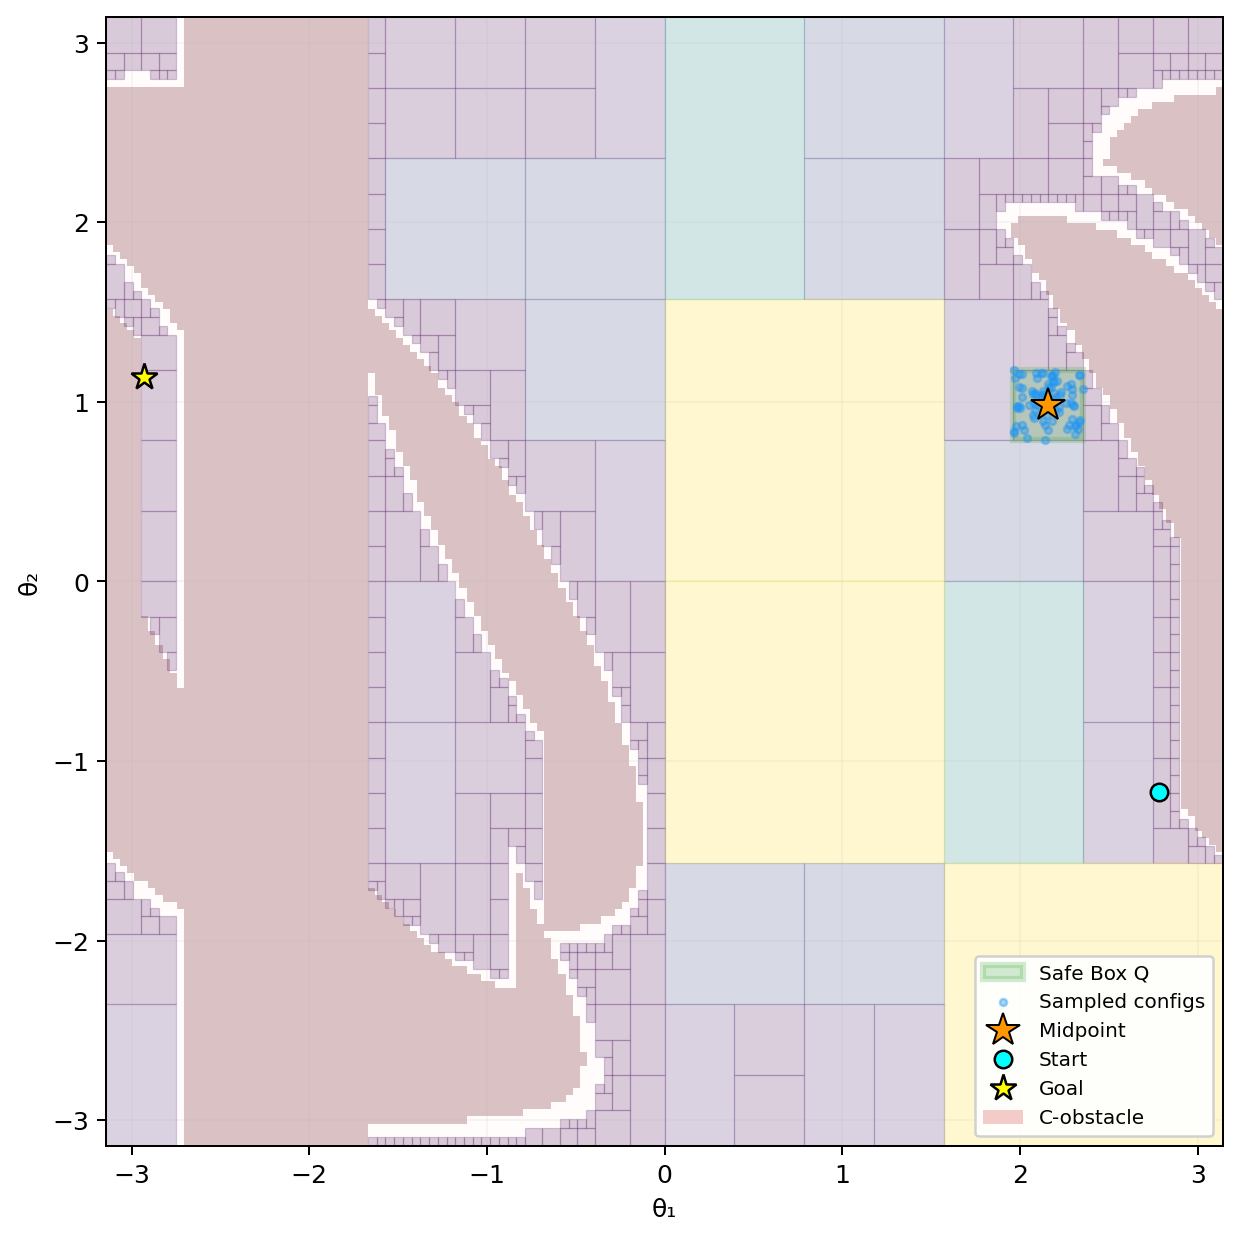
\includegraphics[width=0.325\textwidth]{../sbf_old/figures/sbf_grow_1.png} &
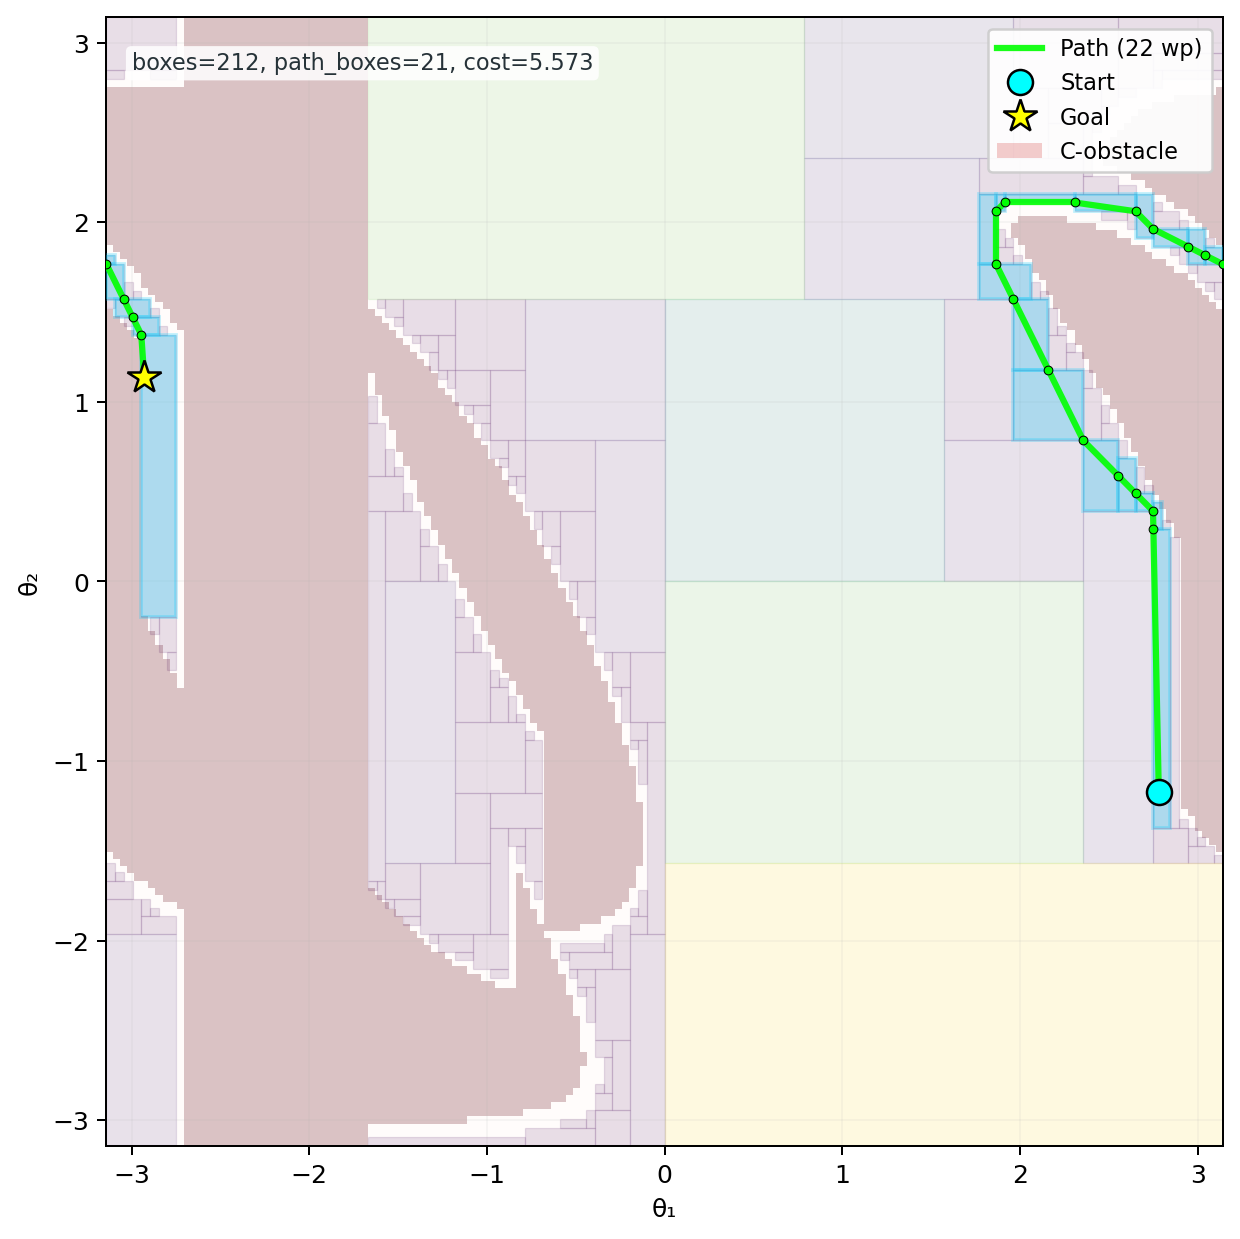
\includegraphics[width=0.325\textwidth]{../sbf_old/figures/sbf_grow_3.png} &
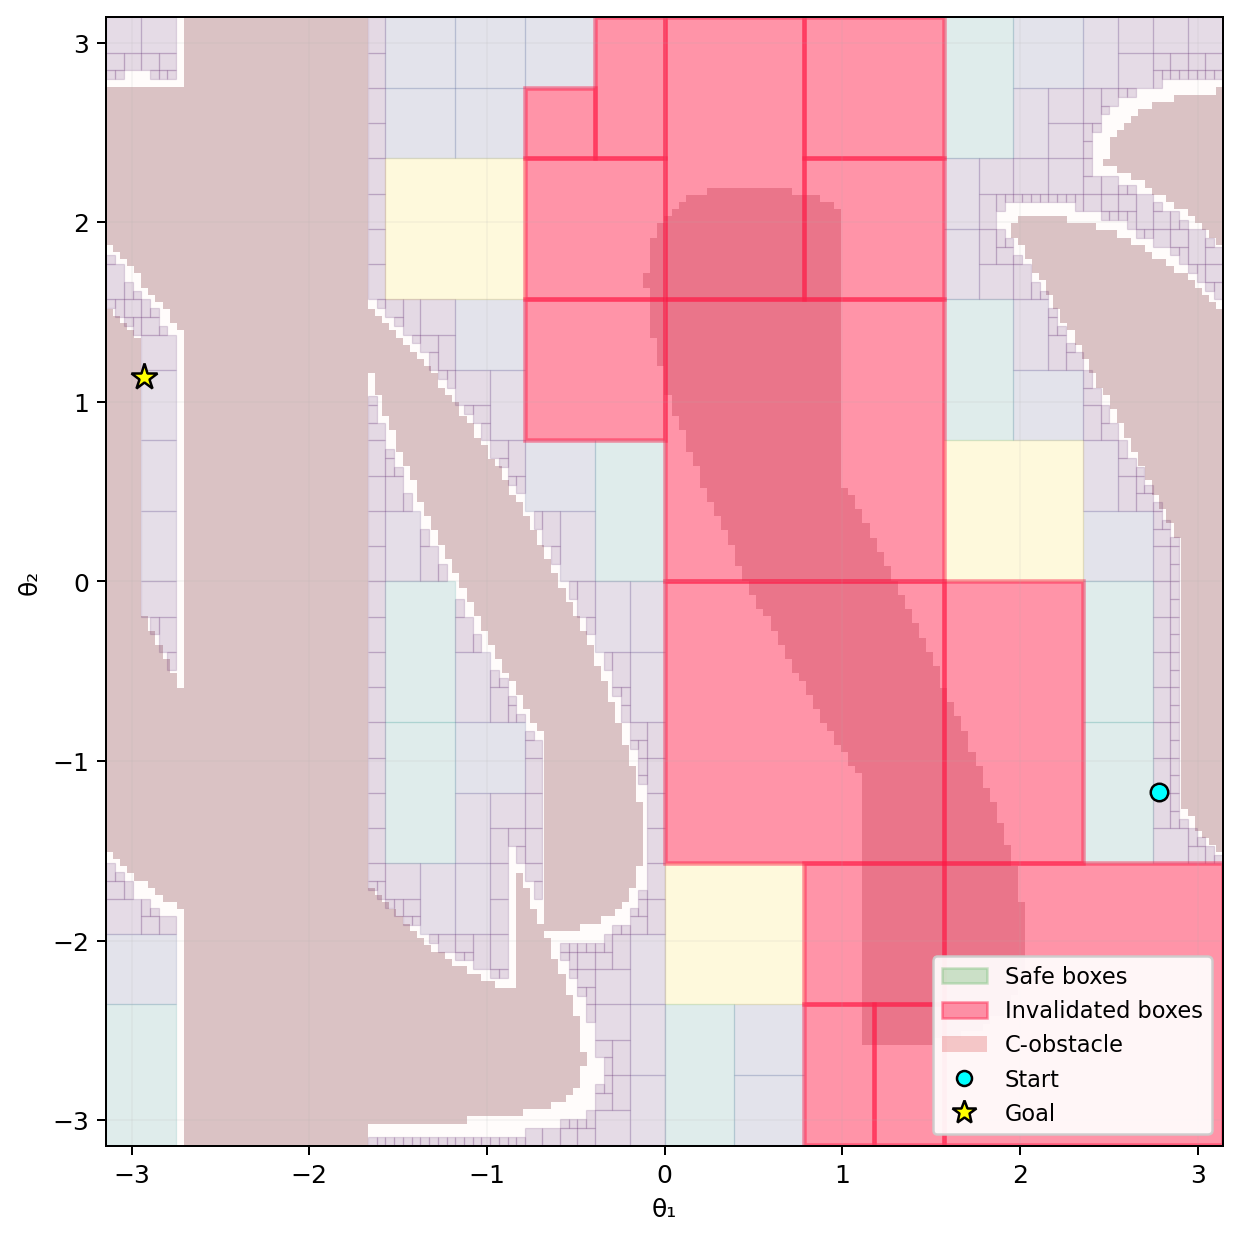
\includegraphics[width=0.325\textwidth]{../sbf_old/figures/sbf_grow_5.png} \\
{\footnotesize (a) C-space cells \& box $Q$} &
{\footnotesize (c) C-space path} &
{\footnotesize (e) Invalidated boxes} \\[4pt]
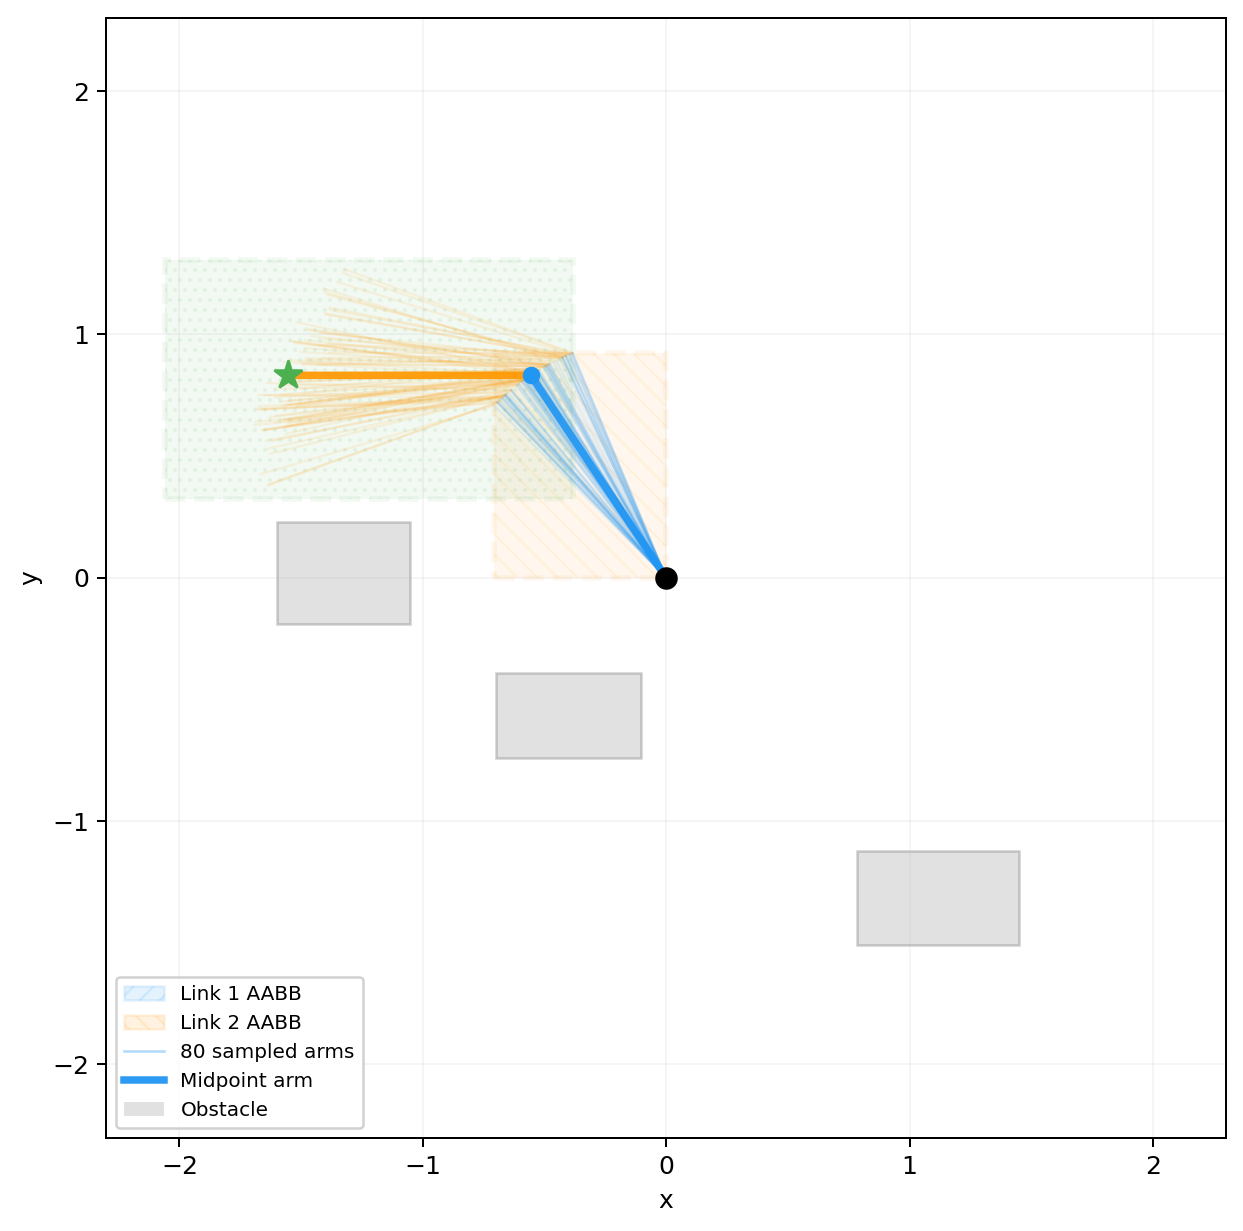
\includegraphics[width=0.325\textwidth]{../sbf_old/figures/sbf_grow_2.png} &
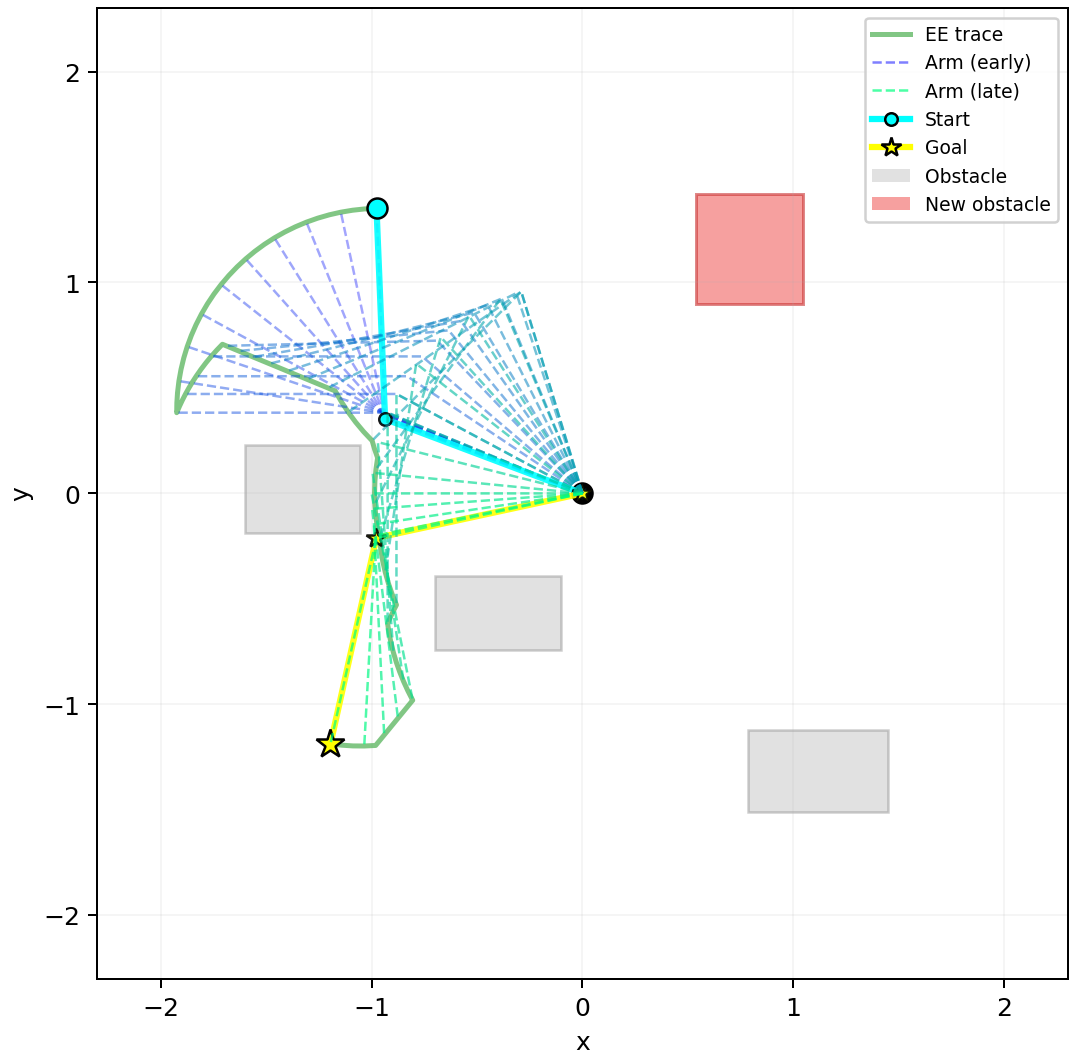
\includegraphics[width=0.325\textwidth]{../sbf_old/figures/sbf_grow_4.png} &
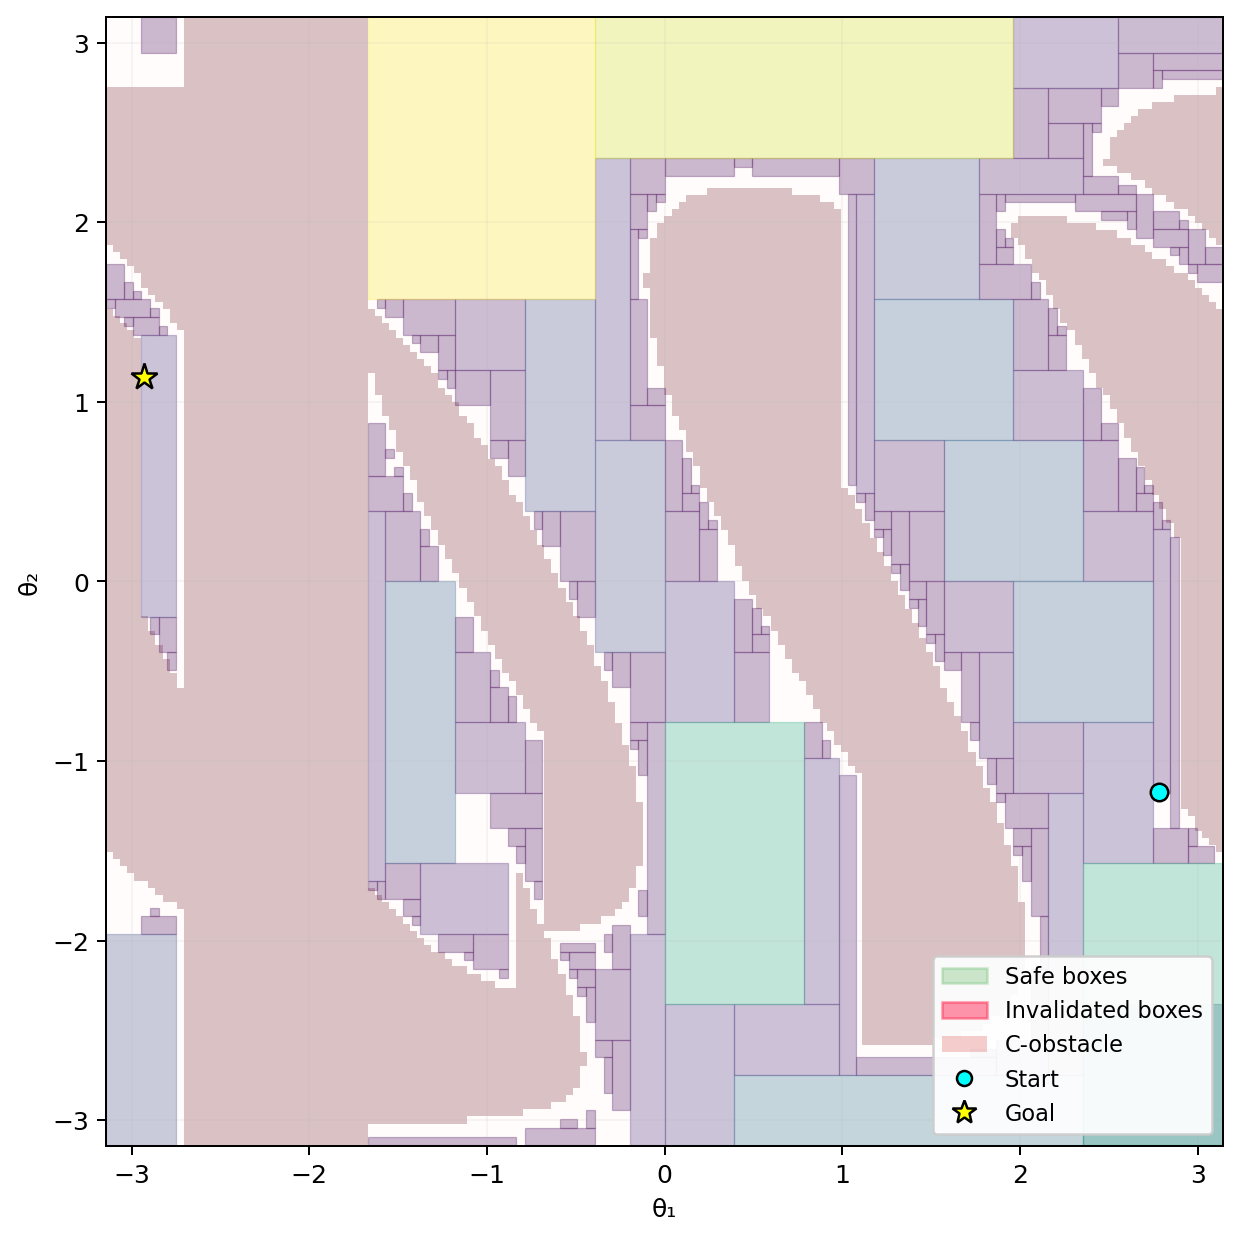
\includegraphics[width=0.325\textwidth]{../sbf_old/figures/sbf_grow_6.png} \\
{\footnotesize (b) Workspace AABBs of $Q$} &
{\footnotesize (d) Workspace path} &
{\footnotesize (f) After regrowth} \\
\end{tabular}
\caption{Illustrative \rbf{} build, query, and obstacle-update cycle on a planar 2-link manipulator.
  (a,\,b)~Adaptive $C$-space cells and workspace AABB envelopes of the highlighted box~$Q$.
  (c,\,d)~Box-corridor path in $C$-space and its workspace trajectory.
  (e,\,f)~After obstacle insertion, intersecting boxes are invalidated (red), and localized repair/regrowth updates the explicit forest without requiring a full rebuild.}
\label{fig:overview}
\end{figure*}

This section describes the planning layer of \rbf{}. The algorithm grows a
scene-specific forest of $C$-space boxes and exports the forest as a graph for
repeated corridor queries. The growth loop is RRT-like, but the state added to
the data structure is a free region rather than a point or edge: samples select
frontiers, the link-envelope oracle materializes a usable box, and accepted
boxes extend a connected region graph. In adaptive cell-decomposition language,
the boxes are cells, FindFreeBox is the local refinement and classification
primitive, and the forest graph is the adjacency structure used for query
search. The link interval envelopes of \cref{sec:link_envelopes} and the
optional LECT cache of \cref{sec:lect} serve this planner as collision-filtering
and materialization tools.

Throughout this section, a validated box means a box accepted by the selected
scene-validation policy. In strict conservative mode, paths that remain inside
the validated box union inherit the corridor statement below. In all reported
planning experiments, paths that leave this union through repair, smoothing, or
external composition are charged where used and passed through the same final
scene audit.

Conceptually, the build process has three stages. First, a seed-guided local
oracle adaptively refines and classifies a $C$-space cell around a selected
configuration. Second, repeated frontier expansion grows these cells into a
connected forest, giving the method its region-valued RRT/PRM character. Third,
consolidation coarsens redundant boxes before the structure is exported as a
query graph. The consolidation pass is part of the reusable build phase and its
time is included in reported build measurements.

\subsection{Construction Objective}\label{sec:forest_objective}

Let $\Q$ denote the joint-limit box and let $\calO$ denote the current obstacle
set. The construction objective is to build a finite family
\[
\mathcal{F} = \{B_1,\dots,B_N\}, \qquad B_i \subseteq \Q,
\]
such that every $B_i$ is a validated free-space box, the union
$\bigcup_i B_i$ covers as much useful query-relevant free space as possible
under the available box, time, and depth budgets, and the induced adjacency
graph supports efficient downstream search. This object is scene-specific:
changing $\calO$ changes which intervals are accepted into the forest, even
though the underlying envelope evidence in LECT remains reusable.

The central structural rule is that the forest is not merely a free-space cover,
but a \emph{corridor-compatible} free-space cover. Boxes are inserted
under a connected-box constraint.

Viewed as adaptive cell decomposition, this objective is intentionally
workload-biased rather than globally exhaustive. The planner does not try to
classify every cell in $\Q$. It refines and accepts cells near useful frontiers,
task seeds, and connector candidates, then keeps the resulting adjacency graph
as the reusable planning object.

\paragraph{Connected-box rule.}
For boxes
\[
B_i = \prod_{d=1}^{n}[l_i^{(d)},u_i^{(d)}],
\qquad
B_j = \prod_{d=1}^{n}[l_j^{(d)},u_j^{(d)}],
\]
\rbf{} treats them as connected when, in every coordinate, the two intervals
either overlap or are separated by at most a small tolerance $\varepsilon_c$:
\[
\max\{l_i^{(d)},l_j^{(d)}\}
\le
\min\{u_i^{(d)},u_j^{(d)}\}+\varepsilon_c,
\qquad d=1,\ldots,n.
\]
When $\varepsilon_c=0$, this reduces to ordinary interval intersection or
boundary touching in every dimension. A small positive tolerance absorbs the
boundary offset used by grower seeds and floating-point roundoff.

This rule is deliberately weaker than requiring a full shared face. It treats
overlap, touching, and tolerance-scale gaps uniformly as graph-connectivity
evidence, while validity remains attached to the accepted box union itself. The
output of the construction stage is a forest of validated boxes whose graph
connectivity is aligned with the corridor object queried later, without imposing
a stricter face-sharing invariant than the grower actually maintains.

\subsection{Find Free Box}\label{sec:forest_ffb}

\textsc{FindFreeBox} descends LECT from the root toward the leaf containing
seed $q\in\Q$, materializing endpoint and link envelopes lazily along the path,
skipping saturated subtrees via occupancy metadata, and returning the current
interval as a validated box candidate as soon as the scene oracle accepts it.
Tree topology and endpoint records are reused from the scene-independent cache,
while scene-specific validation is deferred to each grower visit.
\Cref{alg:ffb_rewrite} gives the complete pseudocode.

\begin{algorithm}[t]
\caption{FindFreeBox: local box materialization around a seed.}
\label{alg:ffb_rewrite}
\footnotesize
\begin{algorithmic}[1]
\REQUIRE Seed configuration $q$, LECT $T$, obstacle set $\calO$, depth cap $D_{\max}$
\ENSURE Validated interval $I_v$ or failure
\STATE $v \gets \mathrm{root}(T)$; $d \gets 0$; initialize current interval and FK state
\WHILE{$d \le D_{\max}$}
  \algcommentline{Cache materialization}
  \STATE materialize the endpoint and link envelopes of $v$ if needed
  \algcommentline{Scene validation}
  \IF{$v$ is marked fully occupied}
    \RETURN failure
  \ENDIF
  \IF{$v$ is validated collision-free with respect to $\calO$}
    \RETURN interval $I_v$
  \ENDIF
  \algcommentline{Refinement}
  \IF{$d = D_{\max}$}
    \RETURN failure
  \ENDIF
  \IF{$v$ has no children}
    \STATE split $v$ along the depth-synchronous split dimension of depth $d$
  \ENDIF
  \STATE $k \gets$ split dimension of $v$
  \STATE $v \gets$ the child of $v$ whose interval contains $q$; update the current interval
  \STATE update the FK state from dimension $k$ onward; $d \gets d+1$
\ENDWHILE
\RETURN failure
\end{algorithmic}
\end{algorithm}

The termination behavior is straightforward. Under depth cap $D_{\max}$, each
loop iteration either returns immediately or descends one more level in the
tree, so the procedure can make at most $D_{\max}+1$ decisions. In strict
conservative mode, any returned interval has passed envelope disjointness
against $\calO$; in performance-oriented modes, the returned interval is a
validated planning region that remains subject to the common final audit used
for reported paths.

\subsection{Forest Growth}\label{sec:forest_growth}

Starting from an initial seed set, the forest is grown by repeatedly invoking
the find-free-box procedure on carefully chosen candidate configurations.
Each seed first produces a root box through the find-free-box procedure, and
these root boxes initialize one or more connected components of the forest.
The main grower should be understood as an evidence-guided rapidly exploring
process rather than as a generic random cover: every iteration chooses a
frontier component, proposes a nearby interval worth testing, and accepts the
result only when it extends the forest by a usable connected corridor segment.

Each iteration makes two explicit heuristic decisions: it samples a target
configuration $q_t$, then chooses a boundary seed on an existing box face that
is closest to that target. The reported planning configuration uses a sequential
Bernoulli schedule with component-connector probability $p_c=0.45$, query-root
bias $p_g=0.20$, intertree-root bias $p_i=0.25$, and unexplored-volume
probability $p_u=0.45$. A component-connector target between disconnected root
components is attempted first. If no connector target is used, coordinated
multi-tree mode may target a root from another active component; because
$p_i\le 0.5$ in the reported runs, no high-bias pulse is active and the
sustained cap is also $0.25$. If no intertree target is used, the grower then
tries a query-root target, then a LECT unexplored-volume leaf, and finally a
uniform root-interval sample. The same reported configuration uses 5000 boxes,
a 60~s build timeout, an FFB depth cap of 120, eight worker threads, a
component-connector candidate limit of four, a staged component-connect radius
of 0.35 in normalized $L_\infty$ distance, a post-connect time budget of
450~ms, and a quality floor of 64 connected boxes. These numbers are planner
settings rather than envelope-theory parameters, but they are part of the
self-contained specification for the reported rows.

Given a target $q_t$ and an existing box
$B=\prod_j[\ell_j,u_j]$, the grower enumerates feasible faces
$f=(B,d,s)$, where $d$ is a joint dimension and $s\in\{-1,+1\}$ is the lower or
upper side. Let $\tau$ be the adjacency tolerance and
$\epsilon_b=\max(\epsilon_{\mathrm{guard}},\tau/4)$. A face is feasible only if
stepping outside it by $\epsilon_b$ remains inside the global root interval. In
the reported configurations $\epsilon_{\mathrm{guard}}=0$, so this formula uses
the $\tau/4$ floor. The
seed associated with the face is
\begin{equation}
q_f[j] =
\begin{cases}
u_d+\epsilon_b, & j=d,\ s=+1,\\
\ell_d-\epsilon_b, & j=d,\ s=-1,\\
\operatorname{clip}(q_t[j],\ell_j+\epsilon_b,u_j-\epsilon_b), & j\ne d,
\end{cases}
\end{equation}
with clipping to $[\ell_j,u_j]$ when a box is thinner than $2\epsilon_b$. Faces
are ranked by the squared target distance
\begin{equation}
  \sigma(f;q_t)=\|q_t-q_f\|_2^2,
\end{equation}
and the implementation retains the 128 lowest-score face candidates across the
scanned frontier boxes. It then tries them in increasing score order, skipping a
candidate if the corresponding LECT leaf is temporarily cooled or if a
component-connection cache has already recorded the same boundary seed. The
first remaining candidate becomes the seed for \textsc{FindFreeBox}.

The candidate box is accepted only if \textsc{FindFreeBox} validates it and the
new box is connected to its parent under the same adjacency predicate used by
the query graph: all dimensions overlap up to tolerance $\tau$, and at least one
dimension touches within tolerance or all dimensions overlap. Failures are also
handled explicitly. When the LECT leaf containing a failed seed reaches the
hard-frontier failure threshold of one failed attempt, the leaf is skipped for a
horizon of 300 subsequently accepted boxes, unless a later depth stage raises
the active search depth and enables a retry. Cooling and the frontier-seed cache
do not alter the validation boundary;
they only reduce repeated calls on already failed or already covered frontier
regions. The resulting method is summarized in \cref{alg:forest_growth}.

\begin{algorithm}[t]
\caption{GrowForest: budgeted expansion of a connected box-region forest.}
\label{alg:forest_growth}
\footnotesize
\begin{algorithmic}[1]
\REQUIRE LECT $T$, obstacle set $\calO$, seed set $\mathcal{S}$, box budget $N_{\max}$, time budget $t_{\max}$
\ENSURE Validated box-region forest $\mathcal{F}$
\STATE $\mathcal{F} \gets \emptyset$; initialize connected components from $\mathcal{S}$
\FORALL{$q \in \mathcal{S}$}
  \STATE $B \gets \procname{FindFreeBox}(q, T, \calO)$
  \IF{$B \neq \emptyset$}
    \STATE insert $B$ into $\mathcal{F}$ as a root box
  \ENDIF
\ENDFOR
\WHILE{$|\mathcal{F}| < N_{\max}$ and time budget not exhausted}
  \STATE draw target $q_t$: connector with prob. $p_c$, query/intertree root with prob. $p_g$ or $p_i$, unexplored LECT leaf with prob. $p_u$, otherwise uniform
  \STATE enumerate feasible faces $f=(B,d,s)$ of frontier boxes and compute $q_f$ and $\sigma(f;q_t)$
  \STATE choose the first of the 128 lowest-score face seeds that is not cooled and not in the frontier-seed cache
  \STATE set $(q_{\mathrm{seed}},B_{\mathrm{near}}) \gets (q_f,B)$ for that face
  \STATE $B_{\mathrm{new}} \gets \procname{FindFreeBox}(q_{\mathrm{seed}}, T, \calO)$
  \IF{$B_{\mathrm{new}} \neq \emptyset$ and $\procname{BoxesConnected}(B_{\mathrm{new}},B_{\mathrm{near}},\tau)$}
    \STATE insert $B_{\mathrm{new}}$ into $\mathcal{F}$; $\procname{UpdateComponents}(\mathcal{F})$
  \ELSE
    \STATE record the failed LECT leaf; cool it after one failed attempt for a 300-box horizon
  \ENDIF
\ENDWHILE
\RETURN $\mathcal{F}$
\end{algorithmic}
\end{algorithm}

The main reported configuration uses coordinated multi-goal growth. Five seed
configurations initialize the shelf roots, and the grower uses the fixed
resource budget defined by the planner configuration. This choice keeps the
growth schedule simple enough to preserve one authoritative forest state while
still exposing reusable LECT evidence across threads and cache-warm reruns. The
regenerated quantitative section in this version focuses on the endpoint
envelope primitive, so this planning configuration is described as the
implementation surface rather than as a reported timing row. The output of this
section is the query-ready box-region object only.

\subsection{Forest Consolidation}\label{sec:forest_consolidation}

Raw growth tends to produce a forest that is finer than necessary. The purpose
of consolidation is to replace a large collection of locally valid
boxes by a smaller collection of equally valid but more useful regions.
Two operations are central.

The first is \emph{promotion}. When two occupied sibling leaves are both
collision-free and their parent interval is also collision-free, the two leaves can be
replaced by the parent. This is the most local form of coarsening and directly
reuses the multiresolution structure of LECT.

The second is \emph{multi-level coarsening}. Exact connected merges are the
cleanest case: if two boxes are connected and their union is itself one box,
the merged region can be accepted directly after validation. More general
connected candidate merges are handled by constructing a candidate parent
region and accepting it only when its chosen envelope representation remains
collision-free against the current obstacle set. This is where the representation choices of
\Cref{sec:link_envelopes,sec:lect} become operational. In an AABB-based forest, the compact parent witness
is typically the enclosing AABB of the two child boxes. In a SupportHull-based
forest, parent witnesses are kept compact only when the merged endpoint-hull
witness remains acceptable; otherwise the child witnesses are kept. Greedy
non-sibling candidates are
ranked by a volume-expansion score, so exact face merges are preferred and
high-inflation parents are deferred unless they pass validation under the
scene oracle. The consolidation logic is summarized in
\Cref{alg:forest_consolidation}.
The final containment-pruning step removes only boxes that are fully covered by
accepted validated regions and whose graph incidence can be transferred to a
selected covering region. It changes neither the represented
free-space union nor the corridor witnesses used by query search.

\begin{algorithm}[t]
\caption{ConsolidateForest: graph-preserving promotion, merging, and pruning.}
\label{alg:forest_consolidation}
\footnotesize
\begin{algorithmic}[1]
\REQUIRE Validated forest $\mathcal{F}$, LECT $T$, obstacle set $\calO$
\ENSURE Consolidated validated forest $\mathcal{F}'$
\STATE $\mathcal{F}' \gets \mathcal{F}$
\algcommentline{Stage 1: sibling promotion}
\REPEAT
  \STATE promote any validated sibling leaves whose parent is collision-free
\UNTIL{no eligible sibling pair remains}
\algcommentline{Stage 2: validated connected/contact merging}
\STATE merge exact connected pairs whose union is itself a single box
\FORALL{connected candidate pairs $(B_i,B_j)$ in $\mathcal{F}'$}
  \STATE build a candidate parent region $H$ and score its volume expansion
  \IF{the chosen envelope representation of $H$ is collision-free with respect to $\calO$}
    \STATE replace $B_i,B_j$ by $H$
  \ENDIF
\ENDFOR
\algcommentline{Stage 3: containment pruning}
\STATE remove only contained boxes whose adjacency and segment witnesses transfer to selected covering regions
\RETURN $\mathcal{F}'$
\end{algorithmic}
\end{algorithm}

Validity follows directly: every accepted promotion or merge has itself passed
the scene oracle, so the represented free-space union cannot shrink.
Containment pruning removes only boxes fully covered by a selected region that
inherits their adjacency witnesses, preserving all corridor connectivity.

\subsection{Corridor Query}
\label{sec:forest_graph}

After growth and consolidation, the forest is exported as a graph
$G=(V,E)$ with one vertex per validated box. Two vertices are connected by an
edge when their boxes satisfy the connected-box rule above. Lightweight querying is possible because this
connected-box structure is enforced during growth and consolidation rather
than repaired after graph export.

If disconnected adjacency islands remain after growth, an optional connector
stage attempts targeted bidirectional sampling bridges between nearest frontier boxes
of different components. A successful bridge is stored as a segment edge rather
than as a claim that the two boxes overlap. This distinction is important for
both the \rbf{} query layer and the GCS negative controls: a segment edge is a
collision-checked path witness between two boxes, whereas a GCS edge over
convex regions requires feasible overlap of the regions themselves.

This pair $(\mathcal{F},G)$ is the final planning object produced by the build
stage. Querying it is intentionally lightweight. Given start and goal
configurations $q_s,q_g$, the planner associates them with start-side and
goal-side boxes in $\mathcal{F}$ and then searches $G$ for a connecting box
sequence. The query problem is reduced to box-corridor
retrieval inside an already constructed free-space representation.

A shortest path on $G$ yields a box sequence whose union defines a corridor
between the two query endpoints. A geometric path is then recovered as a
waypoint chain inside that corridor. In the experiments, this candidate is then
passed through the same OMPL-style simplification/local post-processing and
fixed-step final audit used by the comparison pipelines. That post-processing
can move the final reported path outside the source box union. Consequently,
the box-corridor statement below applies only to contained paths before or after
post-processing, while the reported planning success in the main curves is the
common fixed-resolution audit outcome.

\begin{theorem}[Conditional validated box-corridor path]
\label{thm:corridor_certificate}
Let $\mathcal{F}$ be a forest whose boxes have each passed conservative
link-envelope validation against obstacle set $\calO$. If a continuous path
$\gamma:[0,1]\to\Q$ satisfies
$\gamma([0,1])\subseteq \bigcup_{B\in\mathcal{F}}B$, then every configuration
on $\gamma$ is collision-free with respect to $\calO$.
\end{theorem}

\begin{proof}
For any $s\in[0,1]$, the containment assumption gives a validated box
$B\in\mathcal{F}$ with $\gamma(s)\in B$. By construction, validation of $B$
means every conservative link envelope for $B$ is disjoint from $\calO$.
Because each such envelope contains the link geometry for every configuration
inside $B$ (\cref{sec:link_envelopes}), the robot geometry at $\gamma(s)$ is
also disjoint from $\calO$. Since $s$ was arbitrary, the whole path is
collision-free.
\end{proof}

\paragraph{Reporting protocol.}
\Cref{thm:corridor_certificate} is a conditional statement: it covers path
portions contained in a conservatively validated box union. It is not the
acceptance rule for the main experimental comparisons. When OMPL simplification,
local repair, smoothing, or external composition leaves that union, the path is
accepted only if it passes the same fixed-resolution final scene collision audit
used for the baselines. The main performance curves should therefore be read as
post-processed, fixed-audit planning results rather than as evidence that every
reported path satisfies the box-corridor containment hypothesis.

For dynamic scenes, the same explicit forest representation supports local
graph maintenance without compulsory rebuilds. Each accepted box records the
obstacle evidence that blocked or validated its envelope tests; obstacle
deletions cannot invalidate existing boxes accepted under the same validation
policy, because free space only grows. Deletion triggers only a spatial dirty-region pass around the removed
obstacle to choose local regrowth seeds, after which any new box is validated by
the same oracle as in the original build. Obstacle insertion is stricter: the
new obstacle is inflated by the dirty-region padding, all overlapping boxes are
rechecked exactly, invalid boxes and incident graph edges are removed, and every
surviving segment edge is re-audited in the edited scene. The repair stage then
regrows from deleted-box centers, live neighbours, original task seeds, and
component-boundary candidates; each committed box must pass the active
validation policy before it enters the forest. Finally, query failure can trigger a
bounded local repair search, again filtered by the same final audit. Warm
rebuild remains available as a measured baseline and fallback policy.

% \begin{algorithm}[t]
% \caption{\textsc{IncrementalUpdate}---localized certificate invalidation and graph repair}
% \label{alg:incremental_update}
% \footnotesize
% \begin{algorithmic}[1]
% \REQUIRE Conservative forest $\mathcal{F}$, graph $G$, edited obstacles $\Delta\calO$, LECT $T$
% \ENSURE Repaired forest and adjacency graph, or failure
% \STATE $\mathcal{I} \gets \emptyset$
% \FORALL{$B \in \mathcal{F}$}
%   \IF{the link envelope of $B$ intersects any obstacle in $\Delta\calO$}
%     \STATE add $B$ to invalidated set $\mathcal{I}$
%   \ENDIF
% \ENDFOR
% \STATE remove $\mathcal{I}$ from $\mathcal{F}$ and delete incident graph edges from $G$
% \STATE rebuild connected-box edges among surviving neighbouring boxes
% \IF{localized regrowth is enabled}
%   \STATE seed \textsc{GrowForest} near frontier boxes adjacent to removed regions
%   \STATE accept only boxes conservatively collision-free under the edited scene
% \ENDIF
% \STATE \textbf{return} repaired $(\mathcal{F},G)$ if queried components remain connected; otherwise failure
% \end{algorithmic}
% \end{algorithm}

If no contained conservative corridor is recovered, no box-corridor guarantee
attaches to that query. The construction still exports a concrete box-region
planning object, and \cref{sec:exp} evaluates its build cost, query cost, path
quality, and success rate after the same post-processing and fixed-resolution
final audit used for the other planners.

\section{Experiments}\label{sec:exp}

This section reports the regenerated endpoint-envelope source study
(Experiment~1) and the width-wise link-envelope representation study
(Experiment~2). Together they measure the geometric primitives used by the
later box-validation and planner layers, not planner-level path benchmarks.

\paragraph{Protocol.}
The benchmark uses the IIWA14 model and six fixed joint-box widths
\{0.02, 0.05, 0.10, 0.20, 0.30, 0.50\}~rad. For each width, 1000 shared joint
boxes are generated from the same seeded table and then replayed by all endpoint
sources, giving 6000 endpoint boxes per source. The evaluated sources are IFK
(the public spelling that now subsumes the former AAFK alias), HIFK with depths
3 and 5, CritSample, Analytical, and MC. MC uses width-proportional sample
counts from 2857 to 71429 samples per box, with 50000 reference samples at the
nominal width. The output artifact stores the fixed box table hash so the
link-envelope study can reuse the same corpus.

\paragraph{Metrics.}
For each source and width, the runner records endpoint construction time,
endpoint AABB volume, implementation certification status, and the diagnostic
gap to the finite reference union of CritSample, Analytical, and MC records.
\Cref{tab:exp1_endpoint_envelopes} restores the original Table~I structure and
reports the mean endpoint AABB volume $V$, mean evaluation time, and maximum
observed gap at each fixed width. The gap column is a diagnostic over the
sampled corpus, not a formal containment proof.

\begin{table}[t]
  \centering
  \caption{Endpoint-interval AABB source comparison at fixed widths.}
  \label{tab:exp1_endpoint_envelopes}
  \scriptsize
  \setlength{\tabcolsep}{2.0pt}
  \renewcommand{\arraystretch}{0.76}
  \begin{tabular}{@{}llrrr@{}}
    \toprule
    Width & Source & $V$ (m$^3$) & Mean ($\mu$s) & Max gap (m) \\
    \midrule
    0.02 & IFK & 0.000049 & 4.3 & 0.0000 \\
    0.02 & HIFK\_3 & 0.000047 & 23.9 & 0.0000 \\
    0.02 & HIFK\_5 & 0.000047 & 73.1 & 0.0000 \\
    0.02 & CritSample & 0.000046 & 10.0 & 0.0000 \\
    0.02 & Analytical & 0.000046 & 6475.9 & 0.0000 \\
    0.02 & MC & 0.000029 & 2263.1 & 0.0061 \\
    \addlinespace
    0.05 & IFK & 0.000872 & 4.5 & 0.0000 \\
    0.05 & HIFK\_3 & 0.000784 & 24.1 & 0.0000 \\
    0.05 & HIFK\_5 & 0.000757 & 72.5 & 0.0000 \\
    0.05 & CritSample & 0.000712 & 10.7 & 0.0003 \\
    0.05 & Analytical & 0.000713 & 6609.5 & 0.0000 \\
    0.05 & MC & 0.000499 & 5603.3 & 0.0145 \\
    \addlinespace
    0.10 & IFK & 0.008530 & 4.6 & 0.0000 \\
    0.10 & HIFK\_3 & 0.006907 & 24.1 & 0.0000 \\
    0.10 & HIFK\_5 & 0.006432 & 72.0 & 0.0000 \\
    0.10 & CritSample & 0.005686 & 11.1 & 0.0012 \\
    0.10 & Analytical & 0.005690 & 6753.7 & 0.0000 \\
    0.10 & MC & 0.004201 & 11412.3 & 0.0307 \\
    \addlinespace
    0.20 & IFK & 0.1023 & 4.6 & 0.0000 \\
    0.20 & HIFK\_3 & 0.0676 & 26.4 & 0.0000 \\
    0.20 & HIFK\_5 & 0.0583 & 80.2 & 0.0000 \\
    0.20 & CritSample & 0.0451 & 12.7 & 0.0054 \\
    0.20 & Analytical & 0.0452 & 7074.8 & 0.0000 \\
    0.20 & MC & 0.0351 & 22866.2 & 0.0702 \\
    \addlinespace
    0.30 & IFK & 0.5222 & 4.6 & 0.0000 \\
    0.30 & HIFK\_3 & 0.2819 & 23.4 & 0.0000 \\
    0.30 & HIFK\_5 & 0.2246 & 70.8 & 0.0000 \\
    0.30 & CritSample & 0.1495 & 13.9 & 0.0126 \\
    0.30 & Analytical & 0.1505 & 7218.2 & 0.0000 \\
    0.30 & MC & 0.1202 & 34588.3 & 0.0956 \\
    \addlinespace
    0.50 & IFK & 5.746 & 4.6 & 0.0000 \\
    0.50 & HIFK\_3 & 2.073 & 24.1 & 0.0000 \\
    0.50 & HIFK\_5 & 1.381 & 72.2 & 0.0000 \\
    0.50 & CritSample & 0.6559 & 18.0 & 0.0324 \\
    0.50 & Analytical & 0.6657 & 7489.0 & 0.0030 \\
    0.50 & MC & 0.5476 & 57728.9 & 0.1137 \\
    \bottomrule
  \end{tabular}
\end{table}

\subsection{Endpoint Envelope Source Study}\label{sec:exp_endpoint_envelopes}

\Cref{tab:exp1_endpoint_envelopes} summarizes the endpoint interval-envelope
source comparison used to choose the geometric inputs for the current paper
track. The IFK row now stands for the public spelling whose implementation is
identical to the old AAFK alias, so it is reported only once. IFK remains the
cheapest certified source and stays gap-free against the sampled reference
union over all reported widths, with mean endpoint time between 4.3 and
4.6~$\mu$s.

Hierarchical IFK trades time for tighter certified boxes. All three certified
AA rows remain gap-free against the sampled reference union over the reported
widths. After fixing HIFK's split-policy selection and rerunning the same 6000
shared boxes, HIFK no longer pays the previous online dimension-search
overhead. At width 0.50~rad, the mean endpoint volume drops from 5.746~m$^3$
for IFK to 2.073~m$^3$ for HIFK\_3 and 1.381~m$^3$ for HIFK\_5, while mean
endpoint cost rises from 4.6 to 24.1 to 72.2~$\mu$s. This preserves the same
qualitative trade-off as the old Table~I, but now places HIFK in a practical
middle tier: HIFK\_3 removes most of IFK's wide-box slack, while HIFK\_5 pushes
that trade-off further without the earlier artificial timing plateau.

The non-certified sources are useful as tightness references but are not safe
drop-in replacements for certified validation. CritSample still tracks
Analytical much more closely than any certified AA source on wide boxes,
reaching 0.6559 versus 0.6657~m$^3$ at 0.50~rad while remaining orders of
magnitude cheaper, 18.0 versus 7489.0~$\mu$s, but it exhibits a 0.0324~m maximum
observed gap against the finite reference union. MC is the tightest row at each
reported width, but it is also the slowest and shows the largest observed gap,
reaching 0.1137~m at 0.50~rad. The regenerated Exp.1 result therefore supports
the paper's default design choice: use IFK for cheap certified envelopes, and
reserve hierarchical or sampling-based sources for tighter diagnostics and
future ablation studies.

\subsection{Link-Envelope Representation Study}\label{sec:exp_link_envelopes}

\Cref{tab:tro_link_envelope_widthwise_ifk_s1} restores the original
mainline representation study with the certified IFK\_AA endpoint source and
the fixed short-link split $S=1$. The benchmark reuses the same six fixed
widths and shared box corpus as Experiment~1 and compares only the retained
mainline representations, LinkIAABB and pure SupportHull, on uninflated
short-link record volume, envelope construction time, and envelope-only
obstacle-check time.

% Auto-generated from the width-wise IFK_AA link-envelope representation artifact.
\begin{table}[!t]
\centering
\caption{Width-wise IFK\_AA link-envelope comparison.}
\label{tab:tro_link_envelopes_ifk_s1}
\label{tab:tro_link_envelope_widthwise_ifk_s1}
\scriptsize
\setlength{\tabcolsep}{2.2pt}
\renewcommand{\arraystretch}{0.82}
\begin{tabular}{@{}llrrr@{}}
\toprule
Width & Envelope & $V$ (m$^3$) & Build ($\mu$s) & Collision ($\mu$s) \\
\midrule
0.02 & LinkIAABB & 0.0136 & 0.1 & 0.5 \\
0.02 & SupportHull & 0.000379 & 0.2 & 0.8 \\
\addlinespace
0.05 & LinkIAABB & 0.0199 & 0.1 & 0.5 \\
0.05 & SupportHull & 0.0028 & 0.2 & 0.9 \\
\addlinespace
0.10 & LinkIAABB & 0.0393 & 0.1 & 0.5 \\
0.10 & SupportHull & 0.0151 & 0.2 & 1.1 \\
\addlinespace
0.20 & LinkIAABB & 0.1508 & 0.1 & 0.6 \\
0.20 & SupportHull & 0.1101 & 0.2 & 1.7 \\
\addlinespace
0.30 & LinkIAABB & 0.5193 & 0.1 & 0.8 \\
0.30 & SupportHull & 0.4602 & 0.2 & 2.7 \\
\addlinespace
0.50 & LinkIAABB & 4.691 & 0.1 & 1.1 \\
0.50 & SupportHull & 4.617 & 0.2 & 6.7 \\
\bottomrule
\end{tabular}
\end{table}


The corrected volume proxy tightens monotonically from LinkIAABB to pure
SupportHull at every width. The gap is most visible on narrow boxes: at
0.02~rad the reported volume drops from 0.0136~m$^3$ for LinkIAABB to
0.000379~m$^3$ for SupportHull. As the width grows, the two rows converge, but
the ordering remains unchanged even at 0.50~rad (4.691 versus 4.617~m$^3$).
LinkIAABB remains the cheapest row to construct, staying near 0.1~$\mu$s across
the sweep, while pure SupportHull remains compact at about 0.2~$\mu$s once the
\texttt{keep\_kdop=false} path stops retaining an extra KDOP payload slot. The
obstacle-check time shows the expected mainline trade-off: LinkIAABB stays
cheapest, rising from about 0.5 to 1.1~$\mu$s, while pure SupportHull rises from
about 0.8 to 6.7~$\mu$s as the boxes widen and more survivors reach the GJK
refinement stage. The retained mainline representation set therefore reduces to
a simple coarse-versus-tight trade-off: AABB for the cheapest broad filter, and
pure SupportHull when the tighter directional witness is worth the extra runtime.

\subsection{LECT Disk Microbenchmark}\label{sec:exp_lect_microbench}

Experiment~3 applies the same reopen-per-stage disk benchmark template to the
real Shelf+IIWA persisted cache used by the warm-build study. Each timed stage
reopens the same current-format d18 cache before executing its workload, so the
reported cost is for the persisted LECT path rather than for a database object
left resident by the setup phase. The measured cache stores 524{,}287 nodes and
524{,}287 endpoint-envelope records in a 334.21~MB namespace with 64~KiB node
pages and a 256-page resident cap. To keep the real-cache benchmark bounded,
the read stages sample 2{,}000 persisted operations, checkpoint is measured
after 2{,}000 sampled evidence updates, and compact is measured after
tombstoning 20{,}000 sampled node payloads on a copied sibling namespace.

\begin{table}[t]
  \caption{Disk-backed LECT microbenchmark on the real Shelf+IIWA d18 persisted
  cache. Reported values are average per operation using the most readable unit
  for each row. Checkpoint is measured after 2k sampled evidence updates;
  compact is measured after 20k sampled node tombstones on a copied cache
  namespace.}
  \label{tab:exp3_lect_disk_microbench}
  \centering
  \begin{tabular}{@{}lrr@{}}
    \toprule
    Operation & Ops & Avg. \\
    \midrule
    Open read-only & 1 & 3.894 s \\
    Node box & 2000 & 1.184 ms \\
    Exact box lookup & 2000 & 637.2 $\mu$s \\
    Range query & 2000 & 28.071 ms \\
    Evidence read & 2000 & 3.3 $\mu$s \\
    Checkpoint (2k dirty updates) & 1 & 1.342 s \\
    Compact (20k node tombstones) & 1 & 1.351 s \\
    \bottomrule
  \end{tabular}
\end{table}

\Cref{tab:exp3_lect_disk_microbench} shows that the persisted LECT path is
dominated by whole-store traversal and maintenance once the cache grows to the
full Shelf+IIWA d18 artifact. On this 334.21~MB persisted cache, evidence reads
remain microsecond-scale at 3.3~$\mu$s and exact box lookup stays
sub-millisecond at 637.2~$\mu$s, but node-box fetch rises to 1.184~ms and the
expanded intersecting range-query stage rises to 28.071~ms because it now
traverses a 524k-node disk-backed tree rather than a 511-node synthetic toy.
Reopening the cache costs 3.894~s, while sampled dirty checkpoint and compact
both remain near 1.35~s on copied namespaces. This still matches the design
intent in \cref{sec:lect_storage}: point evidence reuse on reopened persisted
caches is far cheaper than rebuilding the d18 artifact, while heavier storage
maintenance remains an occasional batch cost rather than a per-query tax.

\section{Conclusion}\label{sec:conclusion}

This paper presented \rbf{}, a link-envelope-guided box-forest method for fast
multi-query manipulator planning. Its geometric core maps endpoint interval
envelopes to link interval envelopes via capsule Minkowski decomposition and
convex-hull generator bounding; an RRT-inspired grower builds a scene-specific
box forest into a corridor graph queried by graph search and local refinement;
LECT optionally caches kinematic envelope records to reduce repeated
materialization cost. The regenerated experiments in this version evaluate the
endpoint-envelope primitive directly and add a certified IFK-based $S=1$
link-envelope representation study plus a disk-backed LECT microbenchmark: IFK
is the fastest certified endpoint row, LinkIAABB is the lightest retained link
witness, and the real Shelf+IIWA persisted-cache study shows that evidence
reads stay microsecond-scale, exact box lookup stays sub-millisecond, and
whole-store checkpoint/compact remain second-scale maintenance operations on
the full 524k-node cache. Older planner-level cache,
dynamic-update, and cross-planner tables are intentionally not carried forward.

\paragraph{Limitations.}
The box-corridor guarantee (\cref{thm:corridor_certificate}) is conditional on
conservative IFK validation and path containment inside the validated box union;
the regenerated Exp.1 and Exp.2 rows do not exercise full planner paths and
therefore do not claim that condition. The Exp.1 gap diagnostic is computed
against a finite union of CritSample, Analytical, and MC records, so it should
be read as an implementation sanity check rather than as a formal proof of
containment.

\paragraph{Scope and Future Work.}
The empirical scope in this version covers the endpoint-envelope source sweep,
a width-wise IFK/$S=1$ link-envelope representation study, and a real
Shelf+IIWA persisted-cache microbenchmark. The next steps are to extend the
LECT study from storage-level timings to Shelf+IIWA warm-build rows,
planner-level cache reuse, dynamic-update rows, and broader cross-planner or multi-robot
comparisons under the same fixed-artifact protocol.

\bibliographystyle{IEEEtran}
\bibliography{../sbf_old/references}

\end{document}